\documentclass[notitlepage,aps,prd,nofootinbib]{revtex4-1}
  
\newcommand{\figures}{../outputs/plots}
\newcommand{\includedir}{../latex_files}

%%%%%%%%%%%%%%%%%%%%%%%%%%%%%%%%%%%%%%%%%%%%%%%%%%
% usepackages
\usepackage{amsmath,amssymb,bbm}
\usepackage{graphicx}
\usepackage[protrusion=true,expansion=true]{microtype} % make text fow nice...
\usepackage{verbatim} % verbatim text and comment environment
\usepackage{lmodern} % allowing font sizes at arbitrary sizes
\usepackage[free-standing-units]{siunitx} % units package, see https://www.ctan.org/pkg/siunitx
\usepackage[absolute,overlay]{textpos} % for textblock* absolute positioning 
\TPGrid{100}{100} % make our textpos grid 100 by 100 for easy positioning 
% \TPGrid[20mm,20mm]{100}{100} % default mm grid
%\usepackage[texcoord,grid,gridunit=mm,gridcolor=red!10,subgridcolor=green!10]{eso-pic} % layout grid, mm
%\usepackage{tcolorbox}
%\usepackage{enumitem}
%\usepackage{fancyvrb}
%\usepackage{ulem}
%\usepackage{listings}
\usepackage{overpic}
\usepackage[section]{placeins}

%%%%%%%%%%%%%%%%%%%%%%%%%%%%%%%%%%%%%%%%%%%%%%%%%%
% Include commands, style, colors, and abbreviations
% Load colors for everything!
\makeatletter
\@ifpackageloaded{xcolor}
 {% true
 }{% false
   % \usepackage[usenames,dvipsnames,svgnames,table]{xcolor}
   \usepackage[usenames]{xcolor}
 }
\makeatother

% Colors from https://styleguide.duke.edu/color-palette/

% These are the official colors, and they cannot be modified by the program (ie changing the opacity or saturation)
\definecolor{Duke Blue}{HTML}{001A57}
\definecolor{Blue Devil Blue}{HTML}{0736A4}

% These are the official recommendations for colors to go with the two official Duke colors. PMS is the Pantone Matching system index, so you can search the color to see what it should look like
\definecolor{PMS Black 3}{HTML}{262626}
\definecolor{PMS Cool Gray 11}{HTML}{666666}
\definecolor{PMS Cool Gray 7}{HTML}{B5B5B5}
\definecolor{PMS Cool Gray 3}{HTML}{E5E5E5}
\definecolor{Light Gray}{HTML}{F5F5F5}

% Blues
\definecolor{PMS 294}{HTML}{003366}
\definecolor{PMS 3015}{HTML}{235F9C}
\definecolor{PMS 3005}{HTML}{0680CD}

% Oranges
\definecolor{PMS 166}{HTML}{D75404}
\definecolor{PMS 1805}{HTML}{CC3300}
% \definecolor{PMS 157}{HTML}{F09905}

% Other
\definecolor{PMS 392}{HTML}{728302} % dark green
\definecolor{PMS 390}{HTML}{A1B70D} % light green
\definecolor{PMS 123}{HTML}{FFD960} % light yellow
\definecolor{PMS 2617}{HTML}{993399} % nice violet

% Define colors for Zeppenfeld_hadronization diagram
% \definecolor{zorange}{HTML}{ffd700}
% \definecolor{zpink}{HTML}{ff789e}
% \definecolor{zbrown}{HTML}{a14001}
% \definecolor{zpurple}{HTML}{d100d1}
% \definecolor{zgrey}{HTML}{e6e6e6}

% Define colors for hadronic shower diagram
% \definecolor{hsblue}{HTML}{0e2fff}
% \definecolor{hsred}{HTML}{ff2900}
% \definecolor{hsgreen}{HTML}{009d00}
% \definecolor{hsblack}{HTML}{000000}


% \definecolor{PMS }{HTML}{} % 



\usepackage{tikz}
\usepackage{adjustbox}
% \usepackage{graphicx}

% \includetikz{boxwidth}{tikzname}

\newcommand{\includetikz}[2]{%

% \framebox{ % show the frame around our box, for debugging spacing issues

    \resizebox{#1}{!}{%
      \centering
      \begin{tikzpicture}[remember picture]%
        \pic[anchor=center,draw,scale=1]{#2};%
      \end{tikzpicture}%
    } % end resizebox

%  } % end of framebox

} % end of newcommand

 % my general commands
%%%%%%%%%%%%%%%%%%%%%%%%%%%%%%%%%%%%%%%%%%%%%%%%%%%%%%%%%%%%%%%%%%%%%%%%%%%%%%%%%%%%%%%%%%%%%%%%%%%%
% Turn off revtex4-1 meaningless float warnings
\usepackage{silence} \WarningFilter{revtex4-1}{Repair the float}

%%%%%%%%%%%%%%%%%%%%%%%%%%%%%%%%%%%%%%%%%%%%%%%%%%%%%%%%%%%%%%%%%%%%%%%%%%%%%%%%%%%%%%%%%%%%%%%%%%%%
% Make the revtex4-1 date not have annoying parentheses any more
\usepackage{etoolbox}
\makeatletter
% \frontmatter@RRAP@format is responsible for the parentheses
\patchcmd{\frontmatter@RRAP@format}{(}{}{}{}
\patchcmd{\frontmatter@RRAP@format}{)}{}{}{}
\renewcommand\Dated@name{}
\makeatother

\usepackage[top=1in, bottom=1.25in, left=1.25in, right=1.25in]{geometry}

%%%%%%%%%%%%%%%%%%%%%%%%%%%%%%%%%%%%%%%%%%%%%%%%%%%%%%%%%%%%%%%%%%%%%%%%%%%%%%%%%%%%%%%%%%%%%%%%%%%%
% citation and href links auto-color
% \let\oldcite=\cite                                                              
% \renewcommand{\cite}[1]{\textcolor{Blue Devil Blue}{\oldcite{#1}}}

% \let\oldhref=\href                                                              
% \renewcommand{\href}[2]{\textcolor{Blue Devil Blue}{\oldhref{#1}{#2}}}

% \let\oldurl=\url                                                              
% \renewcommand{\url}[2]{\textcolor{Blue Devil Blue}{\oldurl{#1}{#2}}}



%%%%%%%%%%%%%%%%%%%%%%%%%%%%%%%%%%%%%%%%%%%%%%%%%%%%%%%%%%%%%%%%%%%%%%%%%%%%%%%%%%%%%%%%%%%%%%%%%%%%
% customized title page

%\makeatletter
%\let\insertadvisor\relax
%\newcommand\advisortitle{Advisor}
%\mode<all>
%{
%  \newcommand\advisor[1]{\def\insertadvisor{#1}}
%}
%
%
%\newtoggle{atlasLogo}
%\newtoggle{dukeLogo}
%
%\toggletrue{atlasLogo}
%\toggletrue{dukeLogo}
%
%\defbeamertemplate*{title page}{mydefault}[1][]
%{
%  \vbox{}
%  \vfill
%  \begingroup
%    \centering
%
%    \begin{beamercolorbox}[sep=8pt,center,#1]{title}
%      \usebeamerfont{title}\inserttitle\par%
%      \ifx\insertsubtitle\@empty\relax%
%      \else%
%        \vskip0.25em%
%        {\usebeamerfont{subtitle}\usebeamercolor[fg]{subtitle}\insertsubtitle\par}%
%      \fi%
%    \end{beamercolorbox}%
%
%    \vskip0.8em\par
%
%    \begin{beamercolorbox}[sep=0pt,center,#1]{author}
%      \usebeamerfont{author}\insertauthor
%    \end{beamercolorbox}
%
%    \vskip0.8em\par
%
%    \ifx\insertadvisor\relax\relax\else
%    \begin{beamercolorbox}[sep=0pt,center,#1]{advisor}
%      \usebeamerfont{advisor}\advisortitle:~\insertadvisor
%    \end{beamercolorbox}
%    \fi
%
%    \begin{beamercolorbox}[sep=0pt,center,#1]{institute}
%      \usebeamerfont{institute}\insertinstitute
%    \end{beamercolorbox}
%
%    \begin{beamercolorbox}[sep=0pt,center,#1]{date}
%      \usebeamerfont{date}\insertdate
%    \end{beamercolorbox}\vskip0.5em
%
%  \endgroup
%  \vfill
%
%  \begin{textblock}{90}[0.5,0.5](50,82) % {width}[hanchor, vanchor](hpos, vpos)
%    \begin{columns}
%
%      \iftoggle {atlasLogo} {%
%      \column{.45\textwidth}\centering%
%        \includegraphics[height=1.32cm]{\includedir/logos/ATLAS-Logo-Ref-RGB.pdf}%
%      }{} % end if atlasLogo
%
%      \ifboolexpr { togl {atlasLogo} and togl {dukeLogo} } {%
%        \column{.1\textwidth}\centering%
%      }{} % end if atlasLogo and dukeLogo
%
%      \iftoggle {dukeLogo} {%
%        \column{.45\textwidth}\centering%
%          \includegraphics[height=1.32cm]{\includedir/logos/dukewordmark_vert_001a57.pdf}%
%      }{} % end if dukeLogo
%
%    \end{columns}
%  \end{textblock}
%
%
%}
%\setbeamertemplate{title page}[mydefault][colsep=-4bp,rounded=true,shadow=\beamer@themerounded@shadow]
%\makeatother


 % style setup
% \input{\includedir/latex/abbreviations.tex}

\usepackage[colorlinks=true, urlcolor={Blue Devil Blue}, linkcolor=black, citecolor=black, filecolor=black]{hyperref}

%%%%%%%%%%%%%%%%%%%%%%%%%%%%%%%%%%%%%%%%%%%%%%%%%%
% load tikz pictures
%%%%%%%%%%%%%%%%%%%%%%%%%%%%%%%%%%%%%%%%%%%%%%%%%%%%%%%%%%%%%%%%%%%%%%%%%%%%%%%%%%%%%%%%%%%%%%%%%%%%
% Edge Generation Schematic

\usepackage{tikz}
\usetikzlibrary{shapes} % shapes.arrows
\usetikzlibrary{arrows} % deprecated, should migrate away from o-latex, someday...
\usetikzlibrary{calc}

\tikzset{edgeGen/.pic={

  \pgfmathsetmacro{\textscale}{0.2}
  \tikzstyle{annot} = [scale=\textscale,text centered]
  % \tikzstyle{labeltext} = [scale=0.8,text centered] % its the same at 0.8 but is now easily changeable

  \tikzstyle{ell} = [draw, ellipse, inner sep=7pt, scale=\textscale, text centered]
  \tikzstyle{squa} = [draw, inner sep=8pt, scale=\textscale, text centered]
  \tikzstyle{bigArrow} = [
    single arrow,                  % Shape of the node
    single arrow head extend=20pt, % Actual width of arrow head
    single arrow tip angle=140,    % Adjust arrow tip angle
    inner sep=12pt,                % Separation between node content and node shape
    shape border rotate=270,       % Rotate the arrow shape to point down
    rotate=90,
    draw,
    scale=0.3,
    ]

  \tikzstyle{curveArrow} = [draw, dashed,
                            line width=1pt,
                            line cap=round,
                            scale=\textscale,
                            -latex]


  \node[draw, inner sep=8pt, scale=0.28, text centered, rotate=90] at (-1.05,0) (comm) {PhD Committee $k$};

  \pgfmathsetmacro{\profx}{0}
  \pgfmathsetmacro{\profy}{1}

  \pgfmathsetmacro{\subjectx}{1.9}
  \pgfmathsetmacro{\subjectysep}{0.6}

  \node[squa] at (\profx,\profy) (topName) {Prof. Jane};
  \draw[-] (comm.south) -- (topName.west);

  \node[ell] at (\subjectx,\profy+0.6*\subjectysep) (topNameOrg1) {Chemistry};
  \node[ell] at (\subjectx,\profy-0.6*\subjectysep) (topNameOrg2) {Biochemistry};
  \draw[-] (topName.east) -- (topNameOrg1.west);
  \draw[-] (topName.east) -- (topNameOrg2.west);

  \node[scale=0.4, text centered, rotate=90] at (\profx,0) {\ldots};

  \node[squa] at (\profx,-\profy) (bottomName) {Prof. John};
  \draw[-] (comm.south) -- (bottomName.west);

  \node[ell] at (\subjectx,-\profy+\subjectysep) (bottomNameOrg1) {Biology};
  \node[ell] at (\subjectx,-\profy) (bottomNameOrg2) {Neurobiology};
  \node[ell] at (\subjectx,-\profy-\subjectysep) (bottomNameOrg3) {Biochemistry};
  \draw[-] (bottomName.east) -- (bottomNameOrg1.west);
  \draw[-] (bottomName.east) -- (bottomNameOrg2.west);
  \draw[-] (bottomName.east) -- (bottomNameOrg3.west);


  \node[bigArrow] at (3.45,0) (bigArrow1) {All Combinations};

  \pgfmathsetmacro{\combx}{6.8}
  \pgfmathsetmacro{\comby}{-0.2}
  \pgfmathsetmacro{\combr}{1.45}

  \node[ell] at ({\combx+\combr*cos(72*0+90)}, {\comby+\combr*sin(72*0+90)}) (comb-0) {Chemistry};
  \node[ell] at ({\combx+\combr*cos(72*1+90)}, {\comby+\combr*sin(72*1+90)}) (comb-1) {Biochemistry};
  \node[ell] at ({\combx+\combr*cos(72*2+90)}, {\comby+\combr*sin(72*2+90)}) (comb-2) {Biology};
  \node[ell] at ({\combx+\combr*cos(72*3+90)}, {\comby+\combr*sin(72*3+90)}) (comb-3) {Neurobiology};
  \node[ell] at ({\combx+\combr*cos(72*4+90)}, {\comby+\combr*sin(72*4+90)}) (comb-4) {Biochemistry};

  \foreach \i in {0,...,4}
    \foreach \j in {\i,...,4}
      \draw[dotted, line width=0.7pt] (comb-\i) -- (comb-\j);


  \node[bigArrow] at (9.7,0) (bigArrow2) {Graph};

  \pgfmathsetmacro{\graphx}{11.25}


  \node[ell] at (\graphx,  1) (node-1) {Biochemistry};
  \node[ell] at (\graphx, -1.2) (node-0) {Neurobiology};

  \path (comb-3) -- (comb-4) node (combEdge) [midway] {};

  \draw[-, line width=2pt] (node-0) -- (node-1) node (graphEdge1) [midway] {};
  \node[xshift=6pt, rotate=90, scale=\textscale] at (graphEdge1) {$w=2$};

  \draw[curveArrow] ($ (combEdge.center) + (0.5,-0.5) $) to [out=-48,in=-130] ($ (graphEdge1.center) + (-0.5,-0.5) $);
  \node[annot] at (9.35, -1.4) {$w_{\mathrm{edge}} \mathrel{+}= 1$};


  \draw[-,inner sep=0pt,outer sep=0pt, line width=1pt,line cap=round] ($ (node-1) + (0,0.235) $) to [out=15,in=45,loop,min distance=30pt] ($ (node-1) + (0,0.235) $);
  \node[xshift=4pt, yshift=12pt, rotate=34.5, scale=\textscale] at ($ (node-1) + (0,0.235) $) {$w=1$};


}}



%%%%%%%%%%%%%%%%%%%%%%%%%%%%%%%%%%%%%%%%%%%%%%%%%%%%%%%%%%%%%%%%%%%%%%%%%%%%%%%%%%%%%%%%%%%%%%%%%%%%
% document setup
\makeatletter\hypersetup{
    breaklinks, baseurl=http://, pdfborder=0 0 0, pdfpagemode=UseNone, pdfstartpage=1, bookmarksopen=false, bookmarksdepth=2, % to show sections and subsections
    pdfauthor      = {Matthew Epland}, %
    pdftitle       = {Epland - 2018 Scholars@Duke Visualization Challenge: Methods}, % was including the subtitle as well and I wanted to shorten/tweak it...
    pdfsubject     = {},               %
    pdfkeywords    = {2018 Scholars@Duke Visualization Challenge, 2018, Duke, Interdisciplinary, Network Analysis, Methods}
}\makeatother
%%%%%%%%%%%%%%%%%%%%%%%%%%%%%%%%%%%%%%%%%%%%%%%%%%%%%%%%%%%%%%%%%%%%%%%%%%%%%%%%%%%%%%%%%%%%%%%%%%%%
\begin{document}

\title{Exploring Interdisciplinary Connections in Duke Ph.D.\ Committees\\2018 Scholars@Duke Visualization Challenge}
\author{Matthew\,\,Epland}
\affiliation{Duke University, Durham, NC 27707}
\date{January 22, 2018}

\begin{abstract}
Abstract goes here.%TODO needed in plain text for submission, might not include in final paper
\end{abstract}

\maketitle

\section{Introduction}
This submission to the \href{https://rc.duke.edu/scholars-vis-challenge-2018/}{2018 Scholars@Duke Visualization Challenge} explored the nature of interdisciplinary research at Duke by studying the connections found in Ph.D.\ committees for the academic years of 2013--2017. By combining the committee membership data with the faculty appointments directory, connections between different academic organizations were created and turned into an undirected, weighted graph. From this graph communities of closely connected academic organizations were found via the Louvain method, and the level of interdisciplinary activity of each organization was measured by comparing the relative weights of their external and self connections.

\section{Methods}
\subsection{Constructing the Academic Organizations Graph}
Individual Ph.D.\ committees were identified in the \path{dissertation_committees_2012-2017.xlsx} dataset provided by the Graduate School by computing a unique student/committee ID\footnote{\texttt{\{Student random ID\}\_\{Degree Nbr\}\_\{Compl Term\}\_\{Acad Org\}}}. Incomplete and potentially corrupted committees\footnote{Incomplete committees having less than 4 members and \texttt{1838\_2\_1420\_ELEC\&CMP}} were removed. Using the \path{ScholarsAtDuke_Faculty_October2017.xlsx} dataset provided by Scholars@Duke, committee members were matched to faculty appointments via their Duke unique ID numbers (DUID). At Duke faculty can hold one primary appointment and multiple secondary or joint appointments in other academic organizations\footnote{Administrative appointments and organizations were removed as they did not add to the study of interdisciplinary connections between academic organizations. Many organizational unit numbers were merged to clean the data. Additionally similar, but formally distinct, organizations were merged by hand in order to simplify the number of nodes --- in particular the numerous Medical School subdisciplines.}. Each time a faculty member appeared on a committee they were replaced by all of the academic organizations where they held appointments. From this committee level list of organizations, including duplicates, all possible combinations of two organizations were found. Each combination was saved, along with the degree conferred date, to a list of edges. The final academic organizations graph could then be constructed edge-by-edge, increasing the weight $w$ of a particular edges by $1$ each time it appeared in the list. A schematic representation of this process is provided in Figure~\ref{fig:method_schematic}. The graph building code was written in \texttt{python} using \texttt{pandas} \cite{pandas} for data management and \texttt{networkx} \cite{networkx} for graph operations.

% \vspace{0.15cm}
\begin{figure}[!htb]\centering
  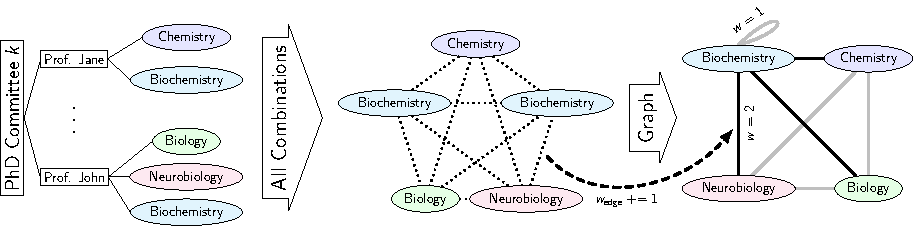
\includegraphics[width=\textwidth]{../poster/tikzout/vis_challenge_2018_poster-matthew_epland-figure0.pdf}
  \caption{Schematic representation of the method used to build the weighted academic organizations graph. Two members from a single committee are illustrated for example, but the method is applied to all committees and all members in practice.}
  \label{fig:method_schematic}
\end{figure}

\subsection{Finding Communities}
The academic organizations graph naturally contains sub-groups, or communities, of related disciplines, such as the Physical Sciences or Liberal Arts. These communities can be constructed algorithmically via the Louvain method \cite{louvain} which optimizes the graph's modularity, a measure of the density of interior to exterior edges of the component communities. The modularity $Q$ of graph $G$ can be defined as in (\ref{eq:modularity}) where $w_{ij}$ is the edge weight between organization nodes $i$ and $j$, $W_{i}$ is the sum of edge weights of node $i$, $W_{\mathrm{G}}$ is the total edge weight of the graph, and $c_{i}$ is the community of node $i$.

\begin{equation} \label{eq:modularity}
Q\left(G\right) = \frac{1}{2 W_{\mathrm{G}}} \sum_{ij \in G} \bigg(w_{ij} - \frac{W_{i} W_{j}}{2 W_{\mathrm{G}}}\bigg) \delta\left(c_{i},\,c_{j}\right)
\end{equation}

In this work the Louvain method was implemented via the \texttt{python-louvain} package \cite{python-louvain} with the resolution parameter\footnote{A resolution of $1$ corresponds to the standard Louvain method, while diverging from $1$ favors communities of different sizes. Other values where tested, but the best results were obtained with a resolution of $1$.} set at the default value of $1$.


\subsection{Measuring Interdisciplinary Activity}
To measure the interdisciplinary activity of each academic organization a straightforward interdisciplinary fraction $f$ of external and self connections was utilized (\ref{eq:intdisfrac}). Here $w_{\text{external}}$ is the sum of external edge weights of an organization's node, while $w_{\text{self}}$ is the weight of the edge from the node to itself. Binning the academic organizations graph by academic year\footnote{With bin edges: 2012--5--1, 2013--8--26, 2014--8--25, 2015--8--24, 2016--8--29, 2017--10--1} it is possible to see how $f$ changes for an organization over time.

\begin{equation} \label{eq:intdisfrac}
f = w_{\text{external}} / \big(w_{\text{external}} + w_{\text{self}}\big)
\end{equation}

$f$ works well for Ph.D.\ granting organizations with good statistics, but frequently breaks down with a value of $f=1.0$ for non-Ph.D.\ granting organizations as they do not have multiple faculty members sitting together on their own Ph.D.\ committees. To help remove such cases from consideration it is required that $w_{\text{total}} = w_{\text{external}} + w_{\text{self}} > 100$ per year, and that an organization have $\geq 3$ such years before being displayed.


\section{Results}
\subsection{Academic Organizations Graph}
% \vspace{0.15cm}
\begin{figure}[!htb]\centering
  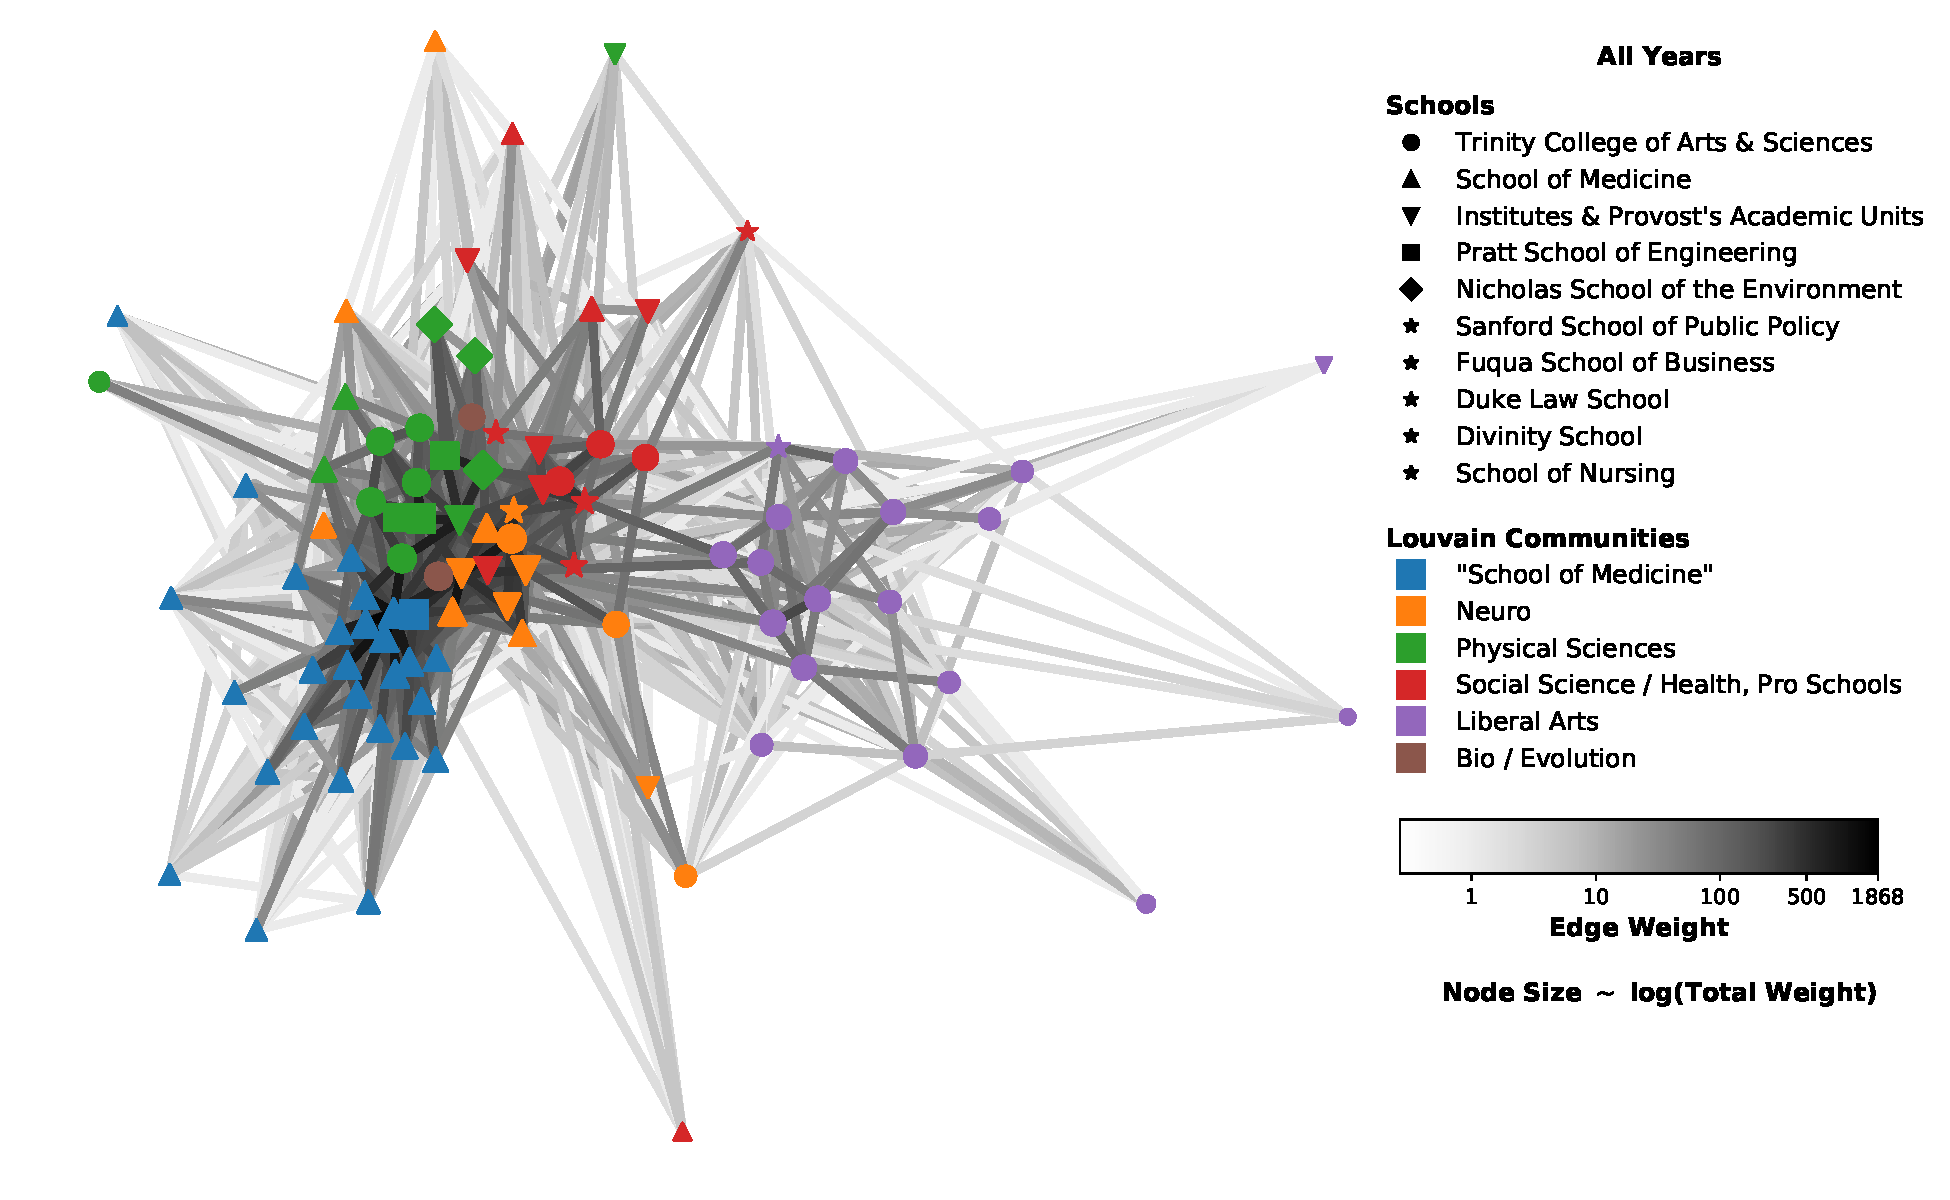
\includegraphics[width=\textwidth]{\figures/network_all_annotated.pdf}
  \caption{Academic organizations graph for all years.}
  \label{fig:graph_all_years}
\end{figure}

% TODO make sure url is correct in the end!
The academic organizations graph for all years may also be viewed interactively online\footnote{\url{http://bl.ocks.org/mepland/raw/ee7d644c613d1ba18289f72d3f1b3456/}}, displayed with the \texttt{visJS2jupyter} \cite{visJS2jupyter} package.

\subsection{Communities}

\subsection{Interdisciplinary Activity}

% TODO reference appendix plots, tables!

\section{Future Improvements}
Improvements.

\section{Conclusions}
Results.

%%%%%%%%%%%%%%%%%%%%%%%%%%%%%%%%%%%%%%%%%%%%%%%%%%%%%%%%%%%%%%%%%%%%%%%%%%%%%%%%%%%%%%%%%%%%%%%%%%%%
%%%%%%%%%%%%%%%%%%%%%%%%%%%%%%%%%%%%%%%%%%%%%%%%%%%%%%%%%%%%%%%%%%%%%%%%%%%%%%%%%%%%%%%%%%%%%%%%%%%%

\bibliographystyle{\includedir/bib/atlasBibStyleWithTitle}
\bibliography{\includedir/bib/bib.bib}

\newpage % TODO hard coded!
%%%%%%%%%%%%%%%%%%%%%%%%%%%%%%%%%%%%%%%%%%%%%%%%%%%%%%%%%%%%%%%%%%%%%%%%%%%%%%%%%%%%%%%%%%%%%%%%%%%%

\appendix*
\section{Louvain Community Members}

% \vspace{0.15cm}
\begin{figure}[!htb]\centering
  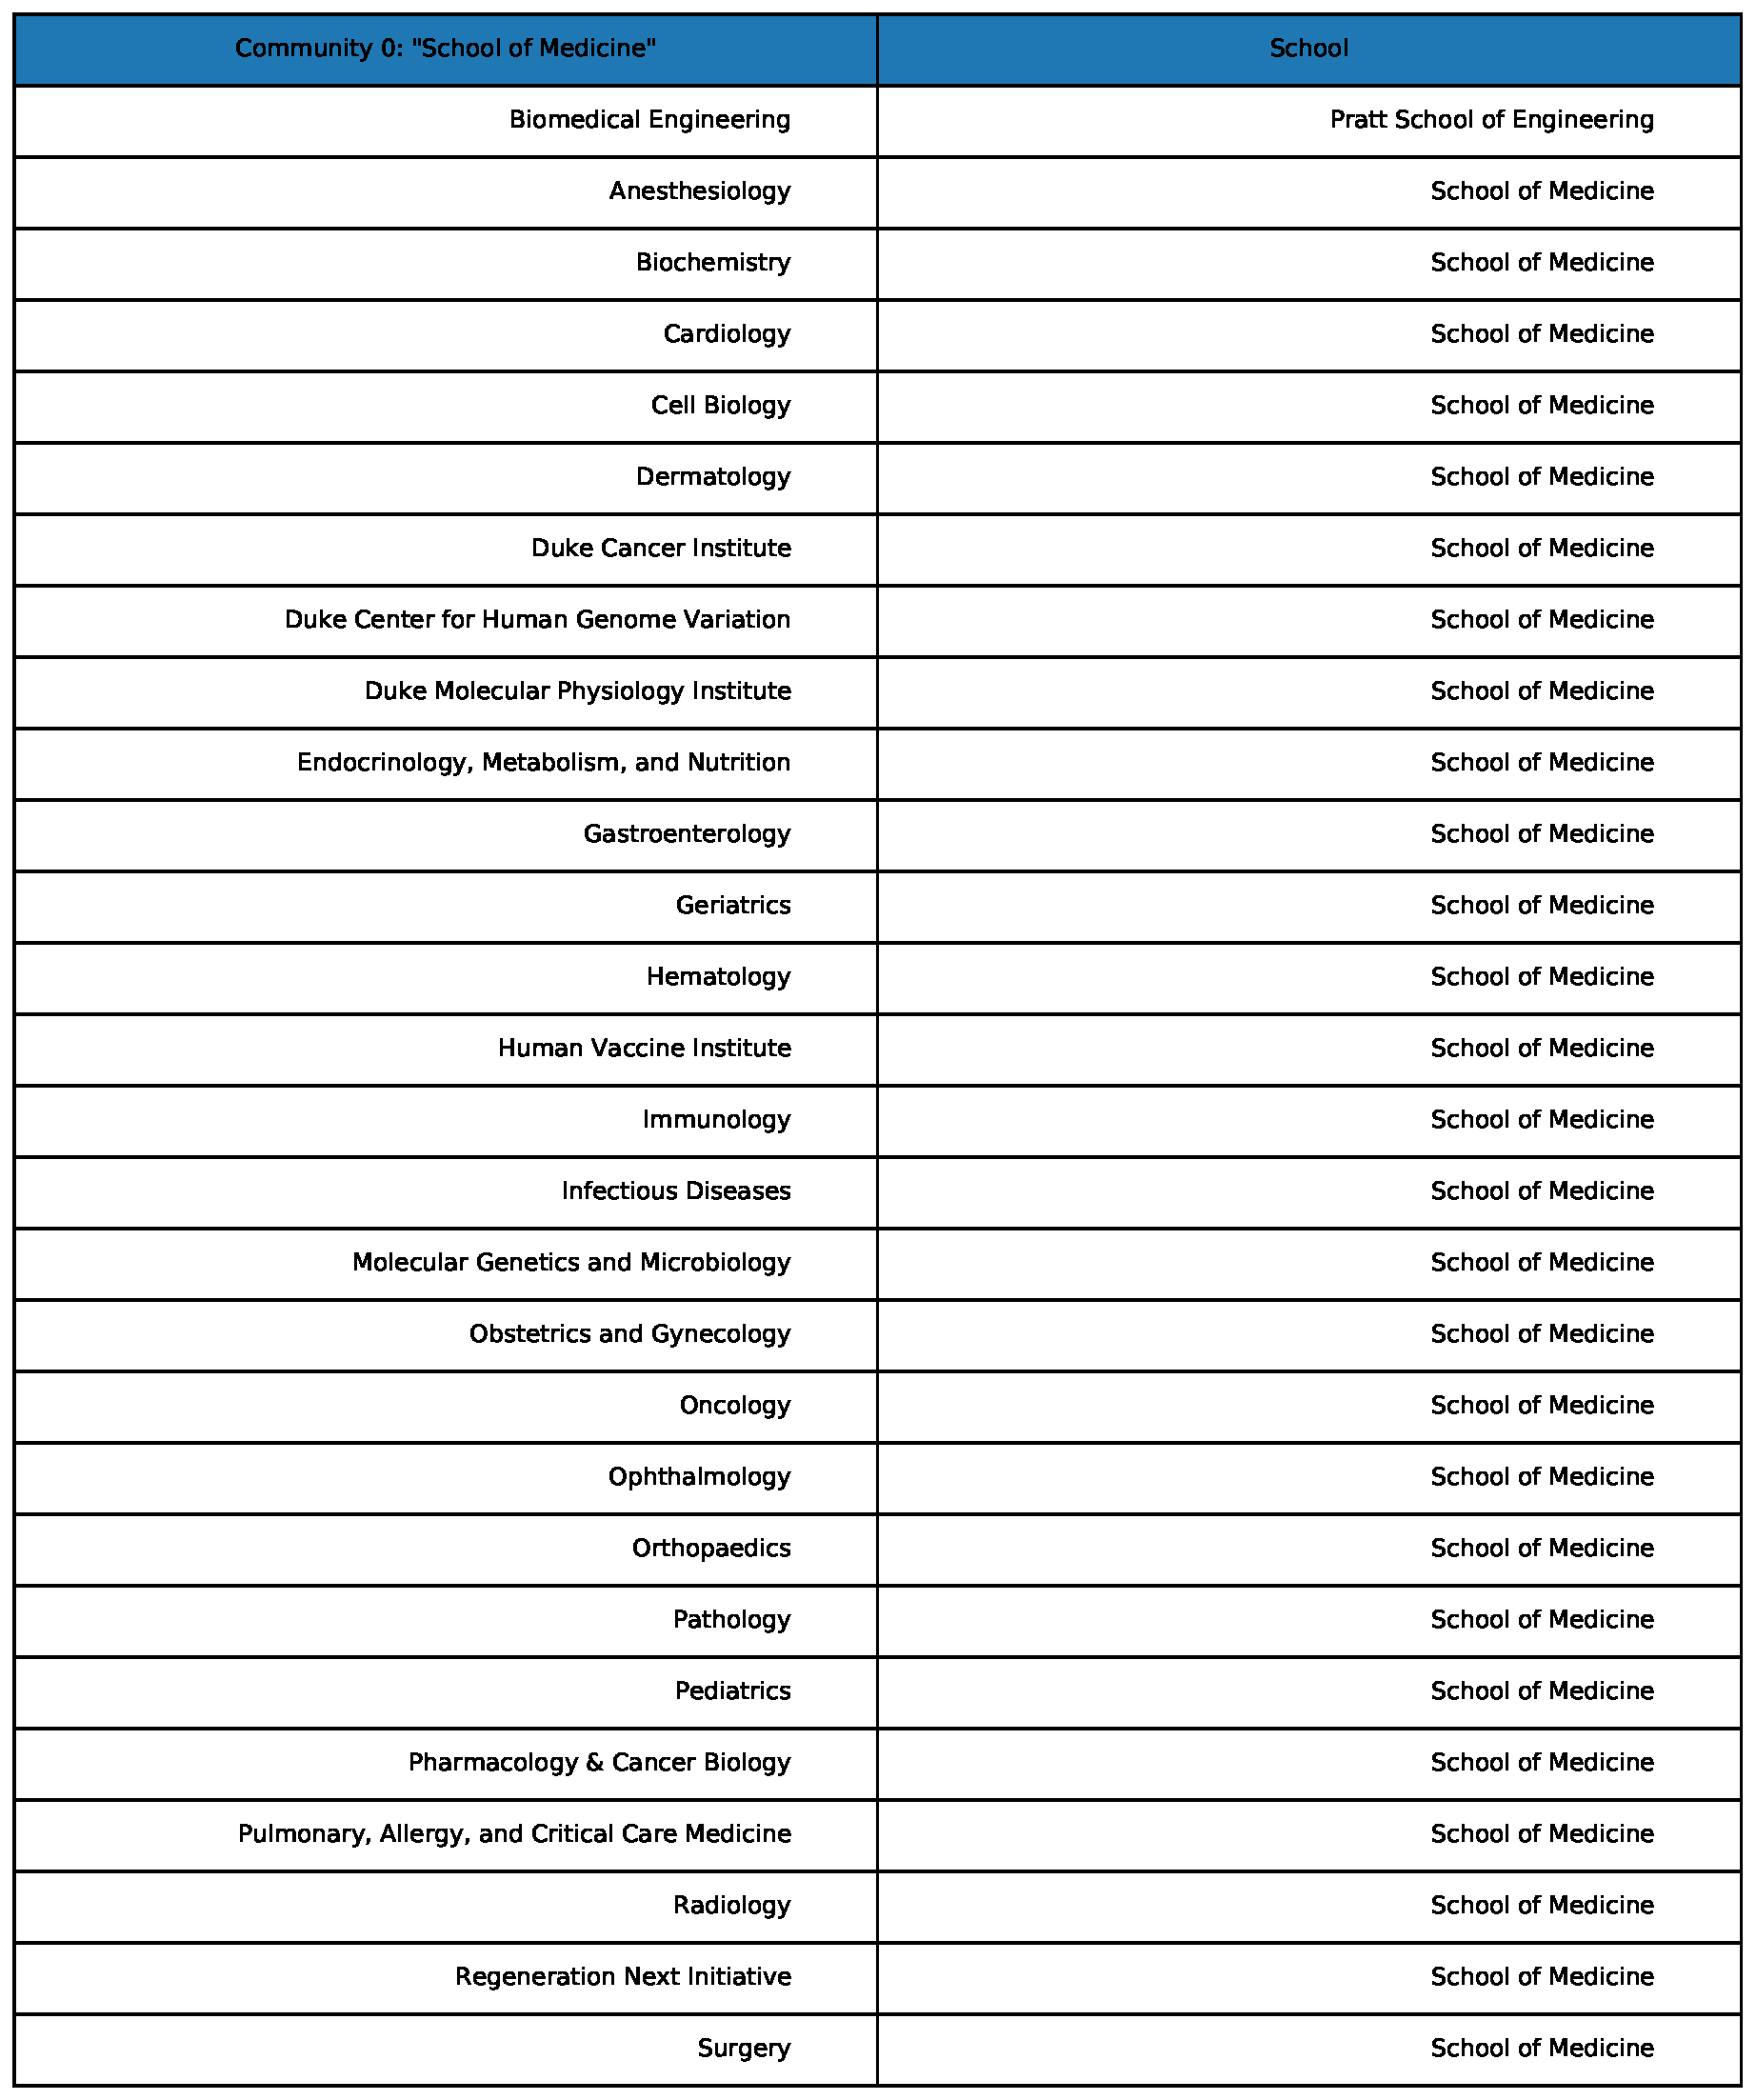
\includegraphics[width=\textwidth]{\figures/community_members/community_0_School_of_Medicine.pdf}
  \caption{Members of the ``School of Medicine" Louvain community.}
  % \label{fig:}
\end{figure}

% \vspace{0.15cm}
\begin{figure}[!htb]\centering
  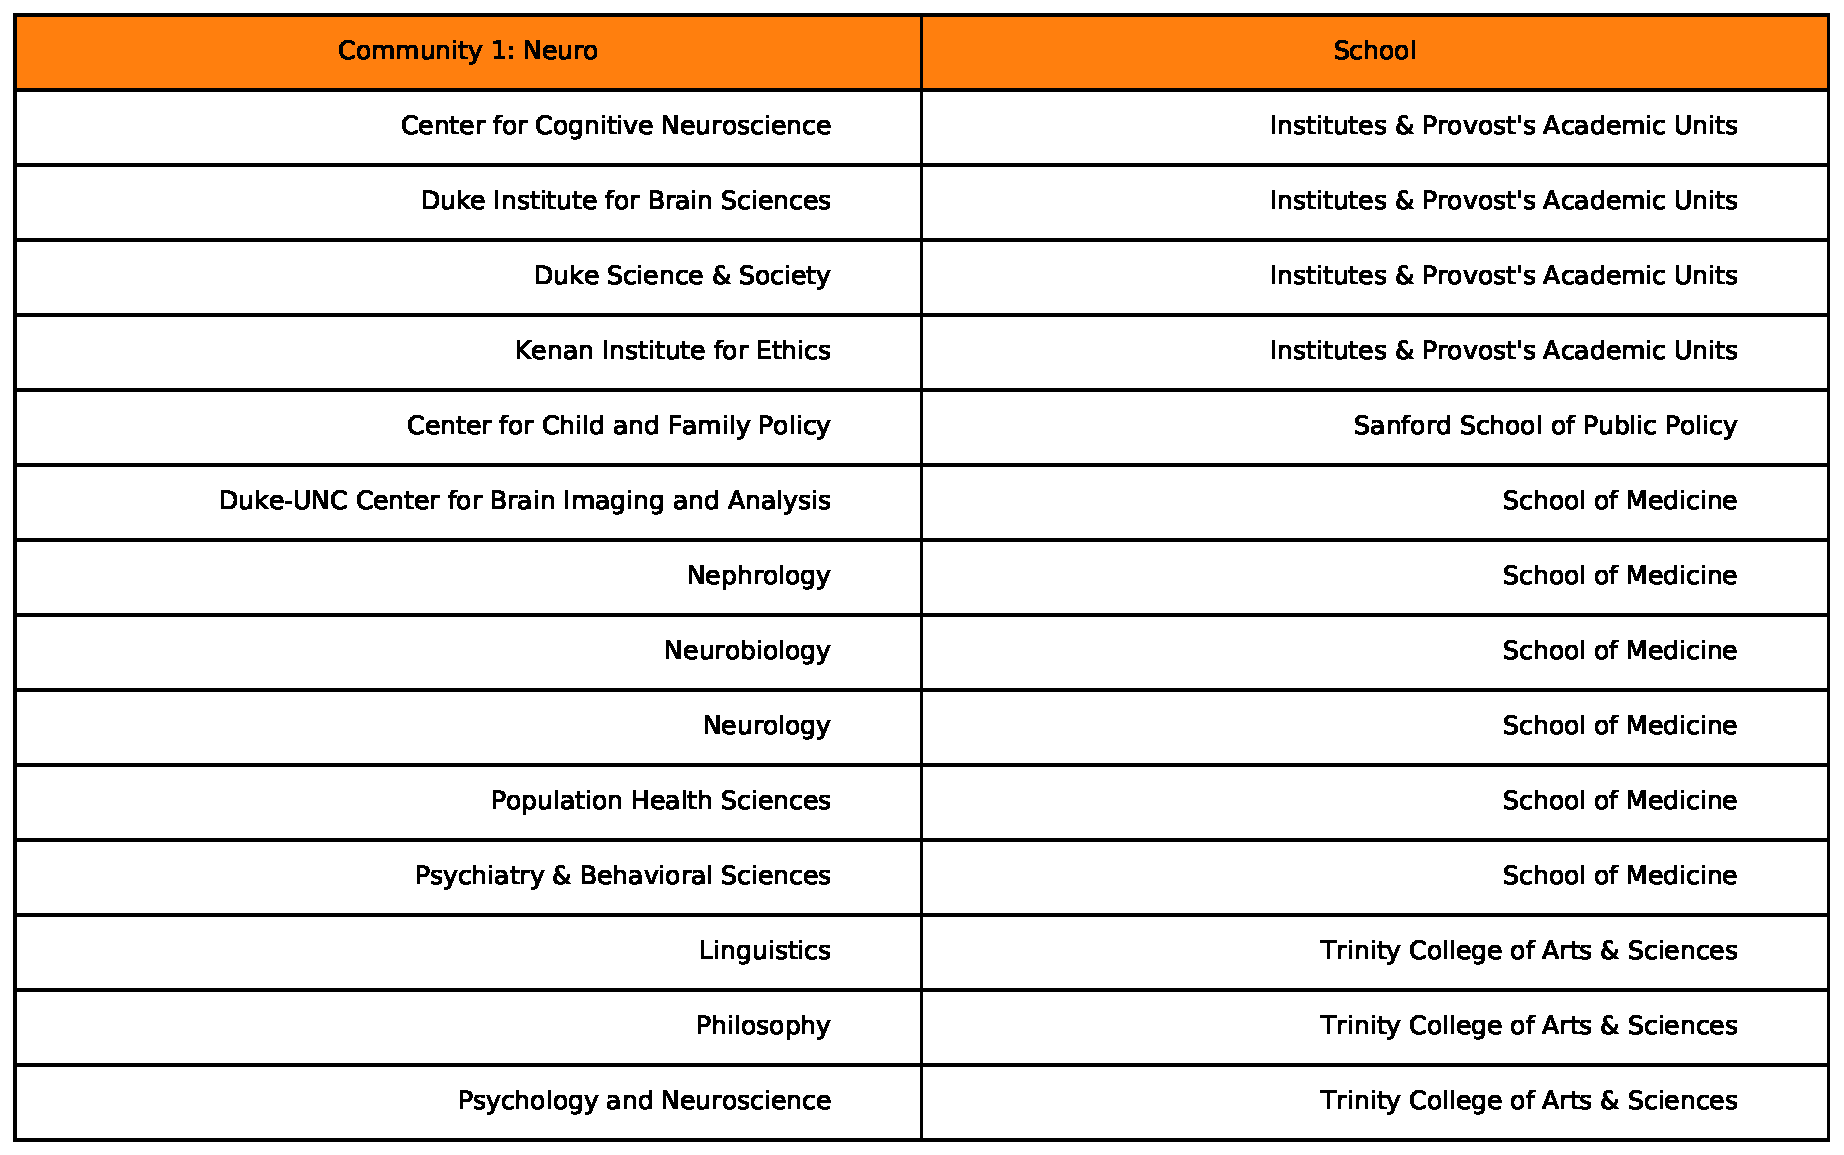
\includegraphics[width=\textwidth]{\figures/community_members/community_1_Neuro.pdf}
  \caption{Members of the Neuro Louvain community.}
  % \label{fig:}
\end{figure}

% \vspace{0.15cm}
\begin{figure}[!htb]\centering
  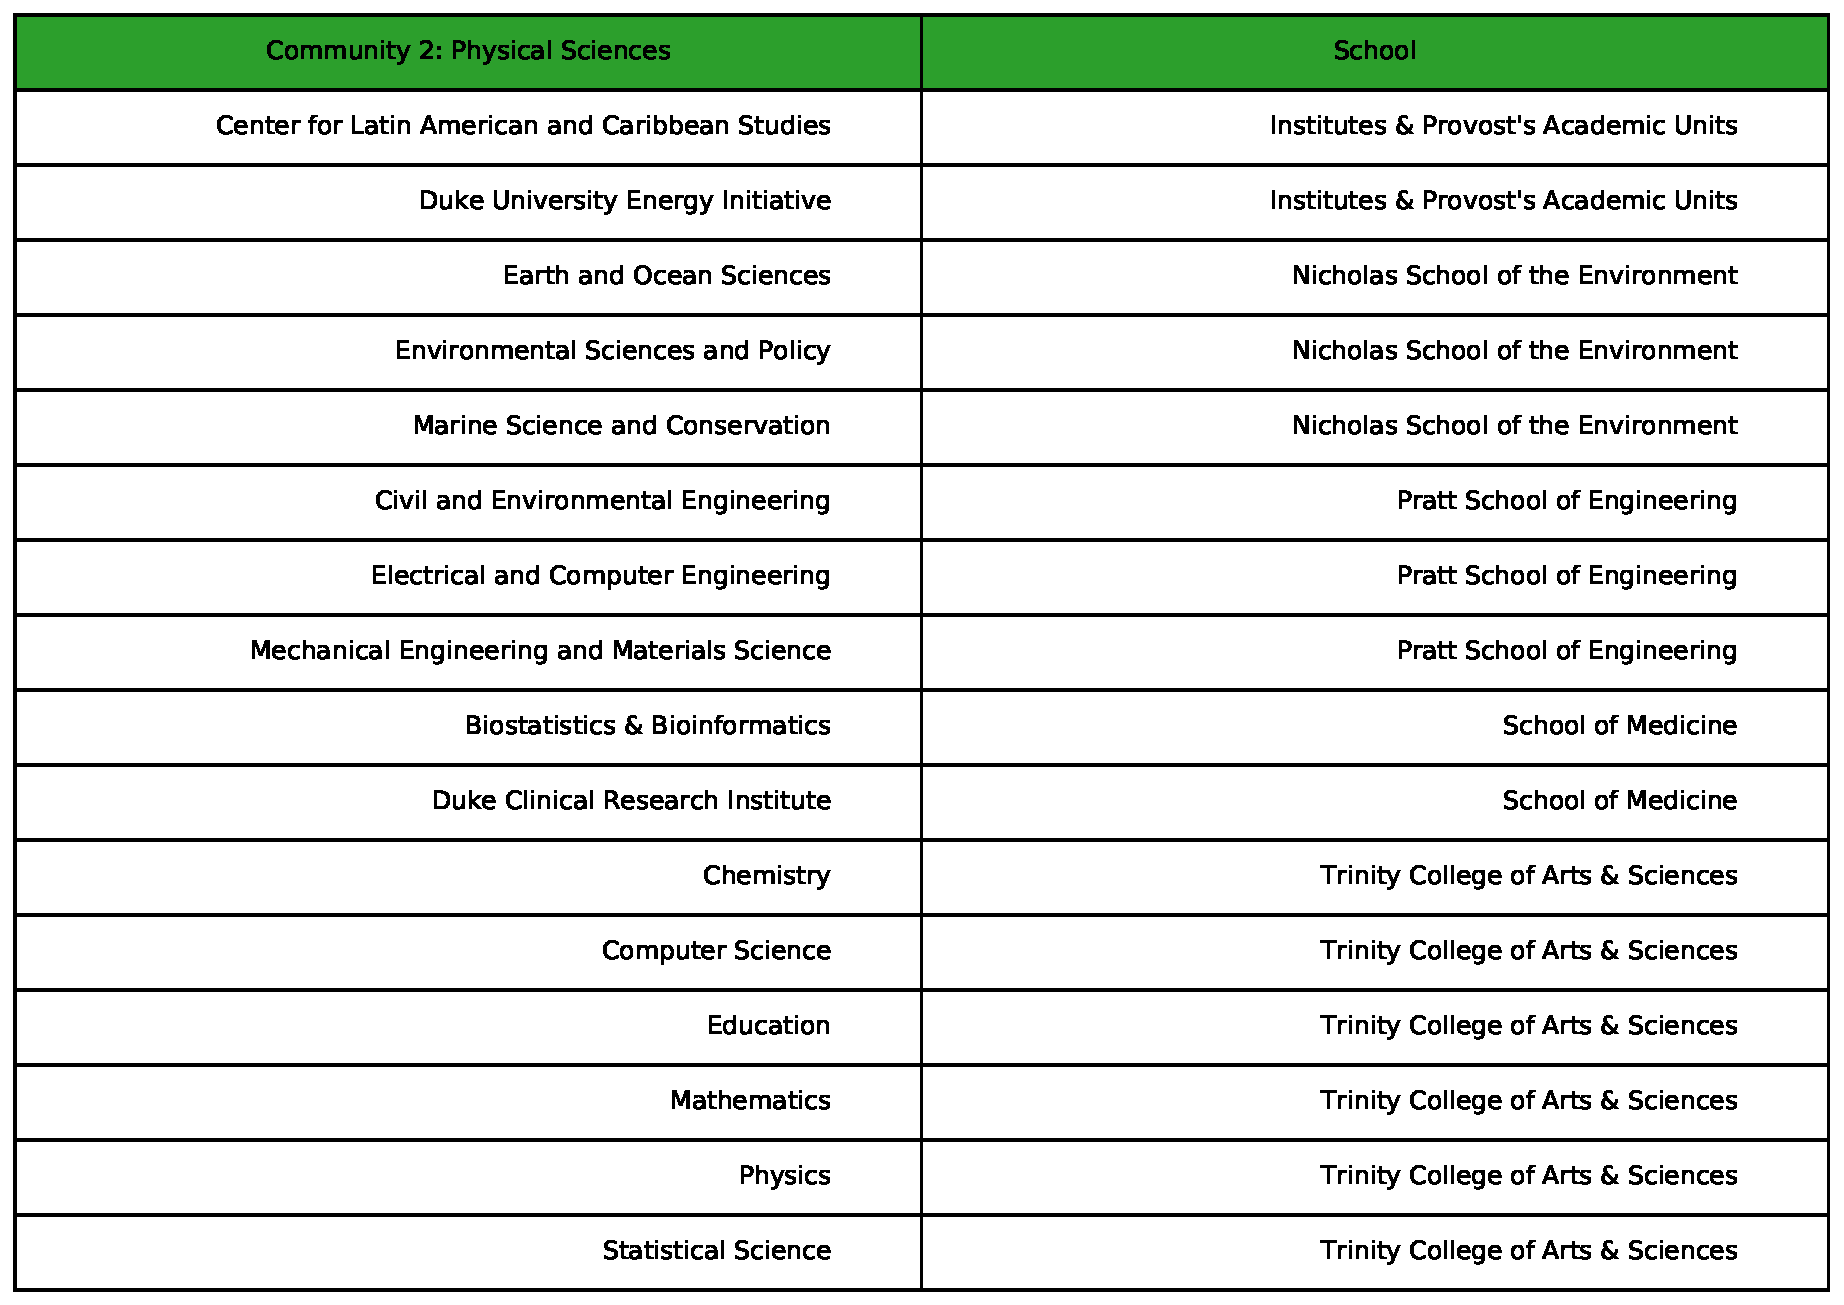
\includegraphics[width=\textwidth]{\figures/community_members/community_2_Physical_Sciences.pdf}
  \caption{Members of the Physical Sciences Louvain community.}
  \label{fig:f_community_physical_sciences}
\end{figure}

% \vspace{0.15cm}
\begin{figure}[!htb]\centering
  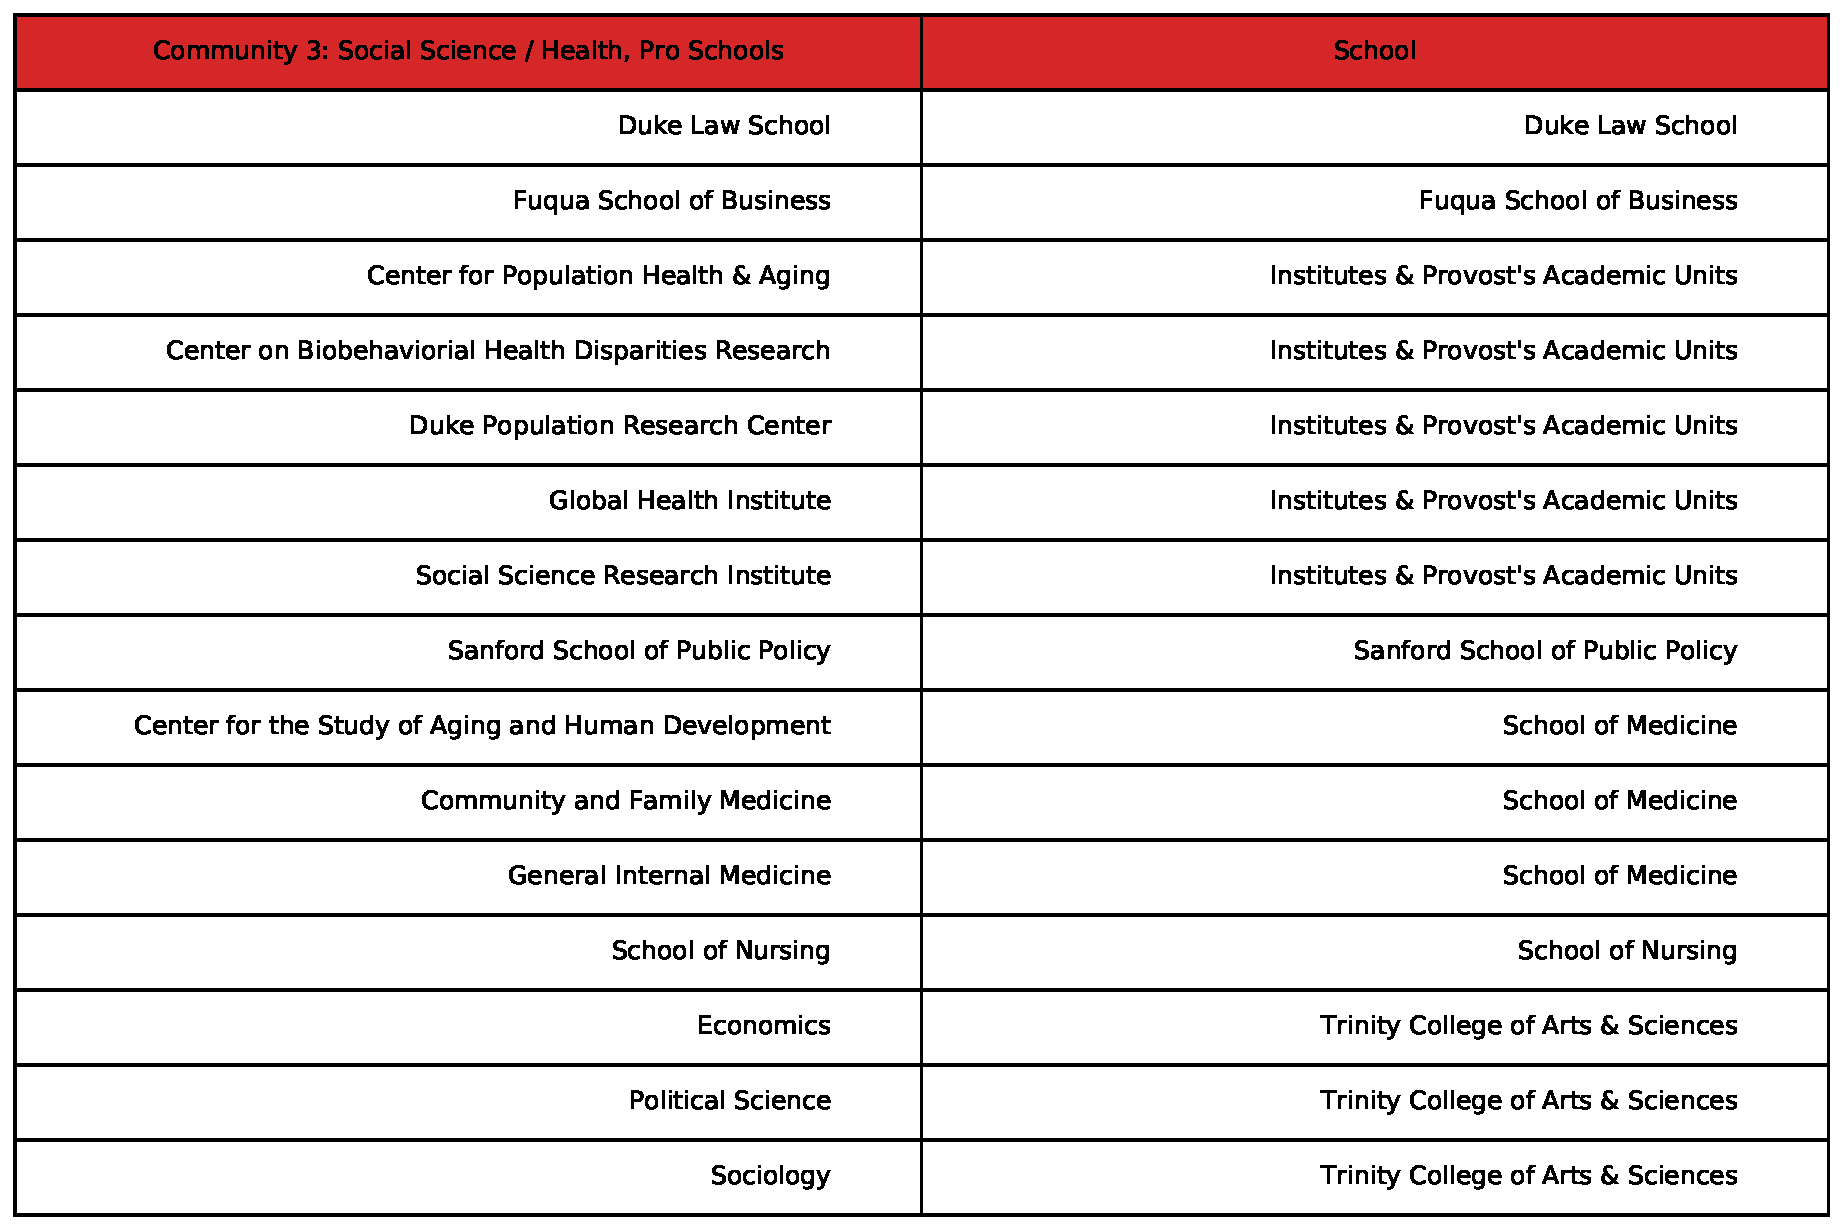
\includegraphics[width=\textwidth]{\figures/community_members/community_3_Social_Science_slash_Health_Pro_Schools.pdf}
  \caption{Members of the Social Science / Health, Pro Schools Louvain community.}
  % \label{fig:}
\end{figure}

% \vspace{0.15cm}
\begin{figure}[!htb]\centering
  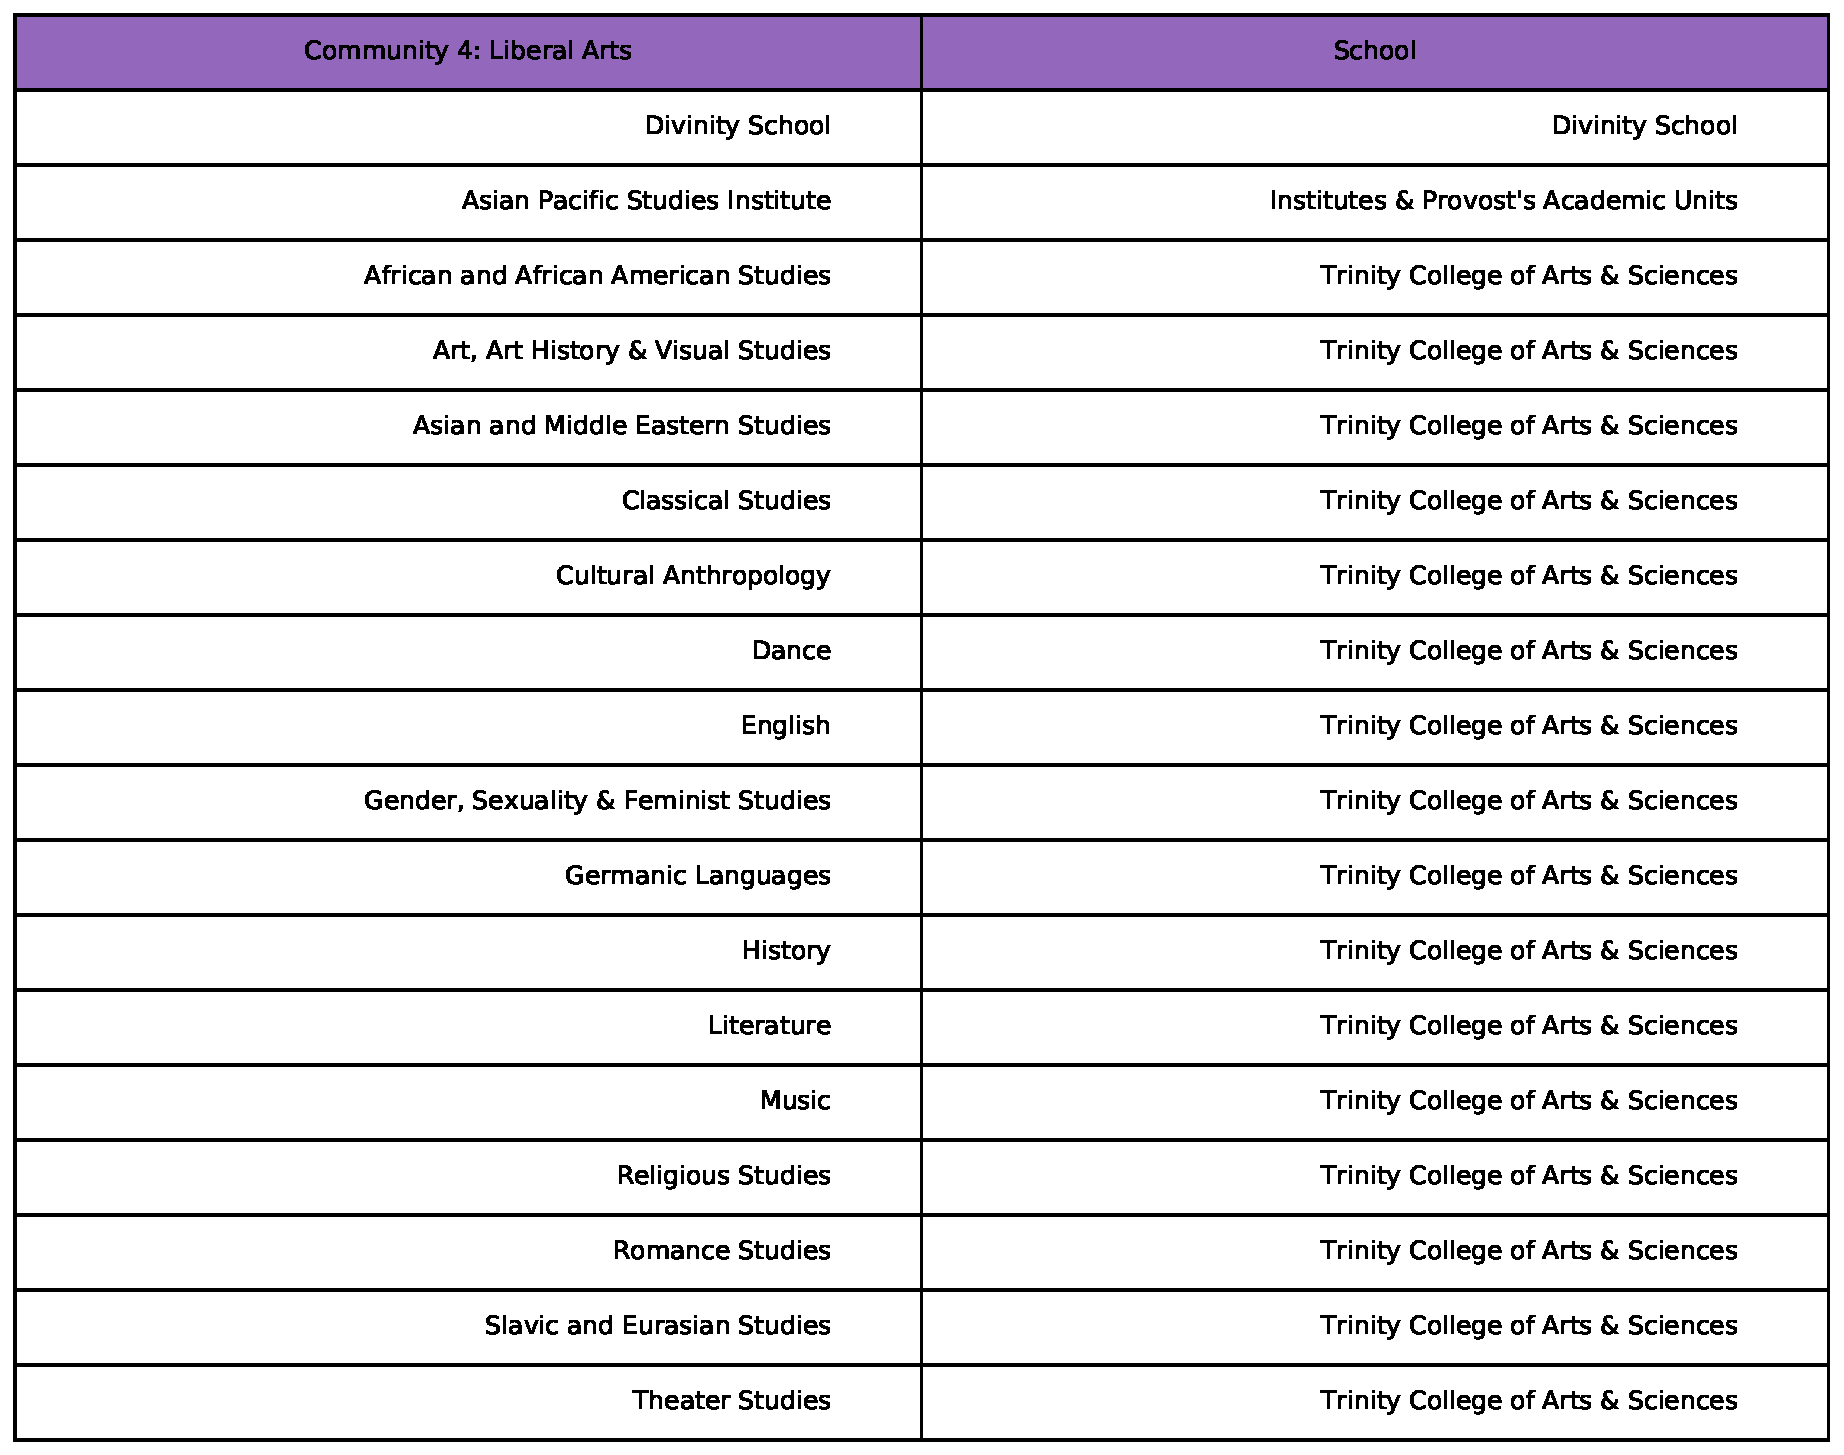
\includegraphics[width=\textwidth]{\figures/community_members/community_4_Liberal_Arts.pdf}
  \caption{Members of the Liberal Arts Louvain community.}
  % \label{fig:}
\end{figure}

% \vspace{0.15cm}
\begin{figure}[!htb]\centering
  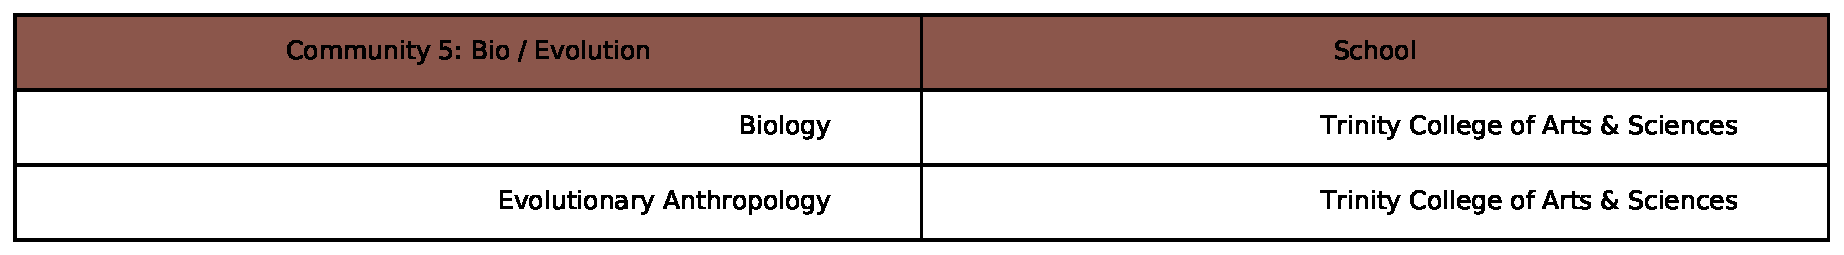
\includegraphics[width=\textwidth]{\figures/community_members/community_5_Bio_slash_Evolution.pdf}
  \caption{Members of the Bio / Evolution Louvain community.}
  % \label{fig:}
\end{figure}


\appendix*
\section{Academic Organizations Graphs by Year}

% \vspace{0.15cm}
\begin{figure}[!htb]\centering
  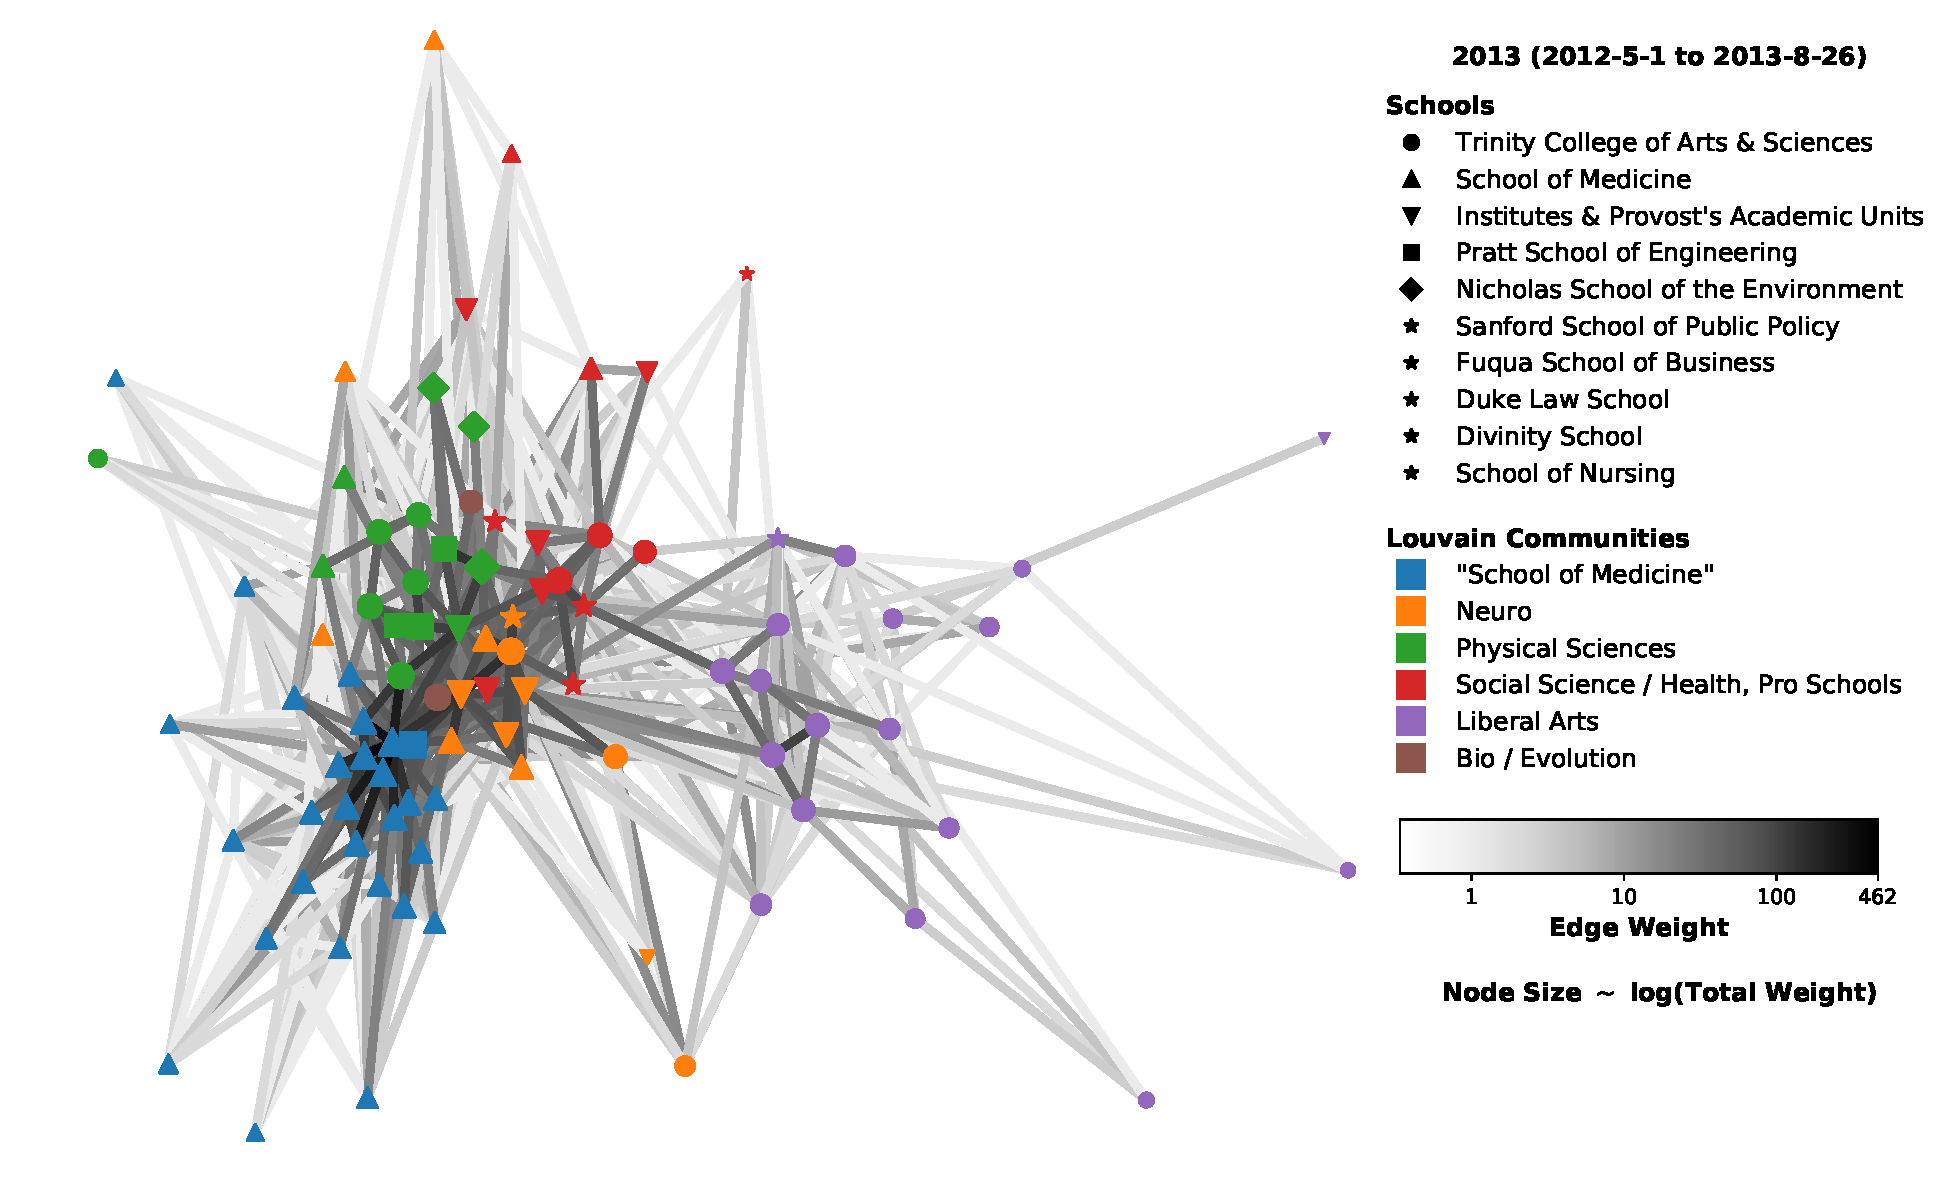
\includegraphics[width=\textwidth]{\figures/time_binned_networks/network_2013.pdf}
  \caption{Academic organizations graph for 2013.}
  % \label{fig:}
\end{figure}

% \vspace{0.15cm}
\begin{figure}[!htb]\centering
  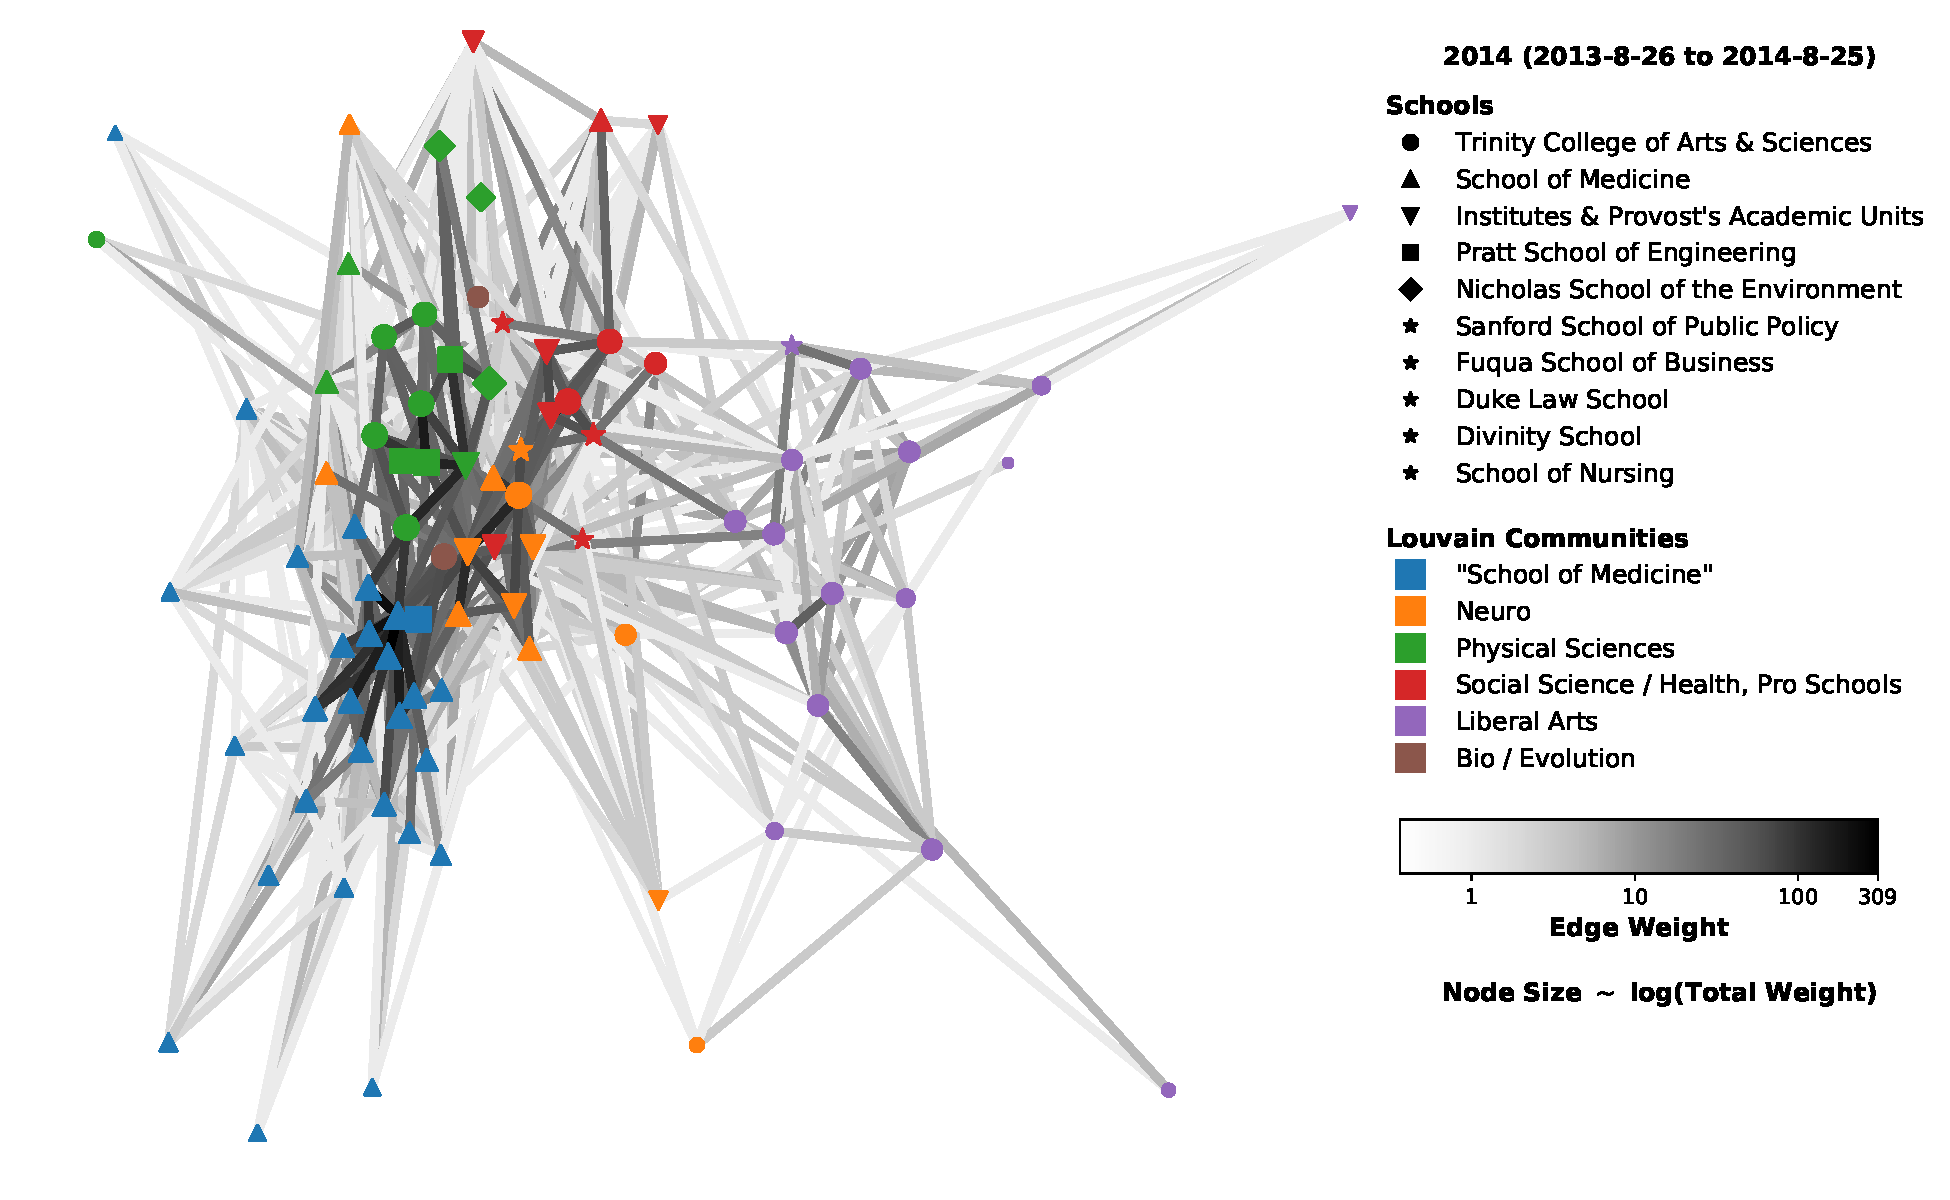
\includegraphics[width=\textwidth]{\figures/time_binned_networks/network_2014.pdf}
  \caption{Academic organizations graph for 2014.}
  % \label{fig:}
\end{figure}

% \vspace{0.15cm}
\begin{figure}[!htb]\centering
  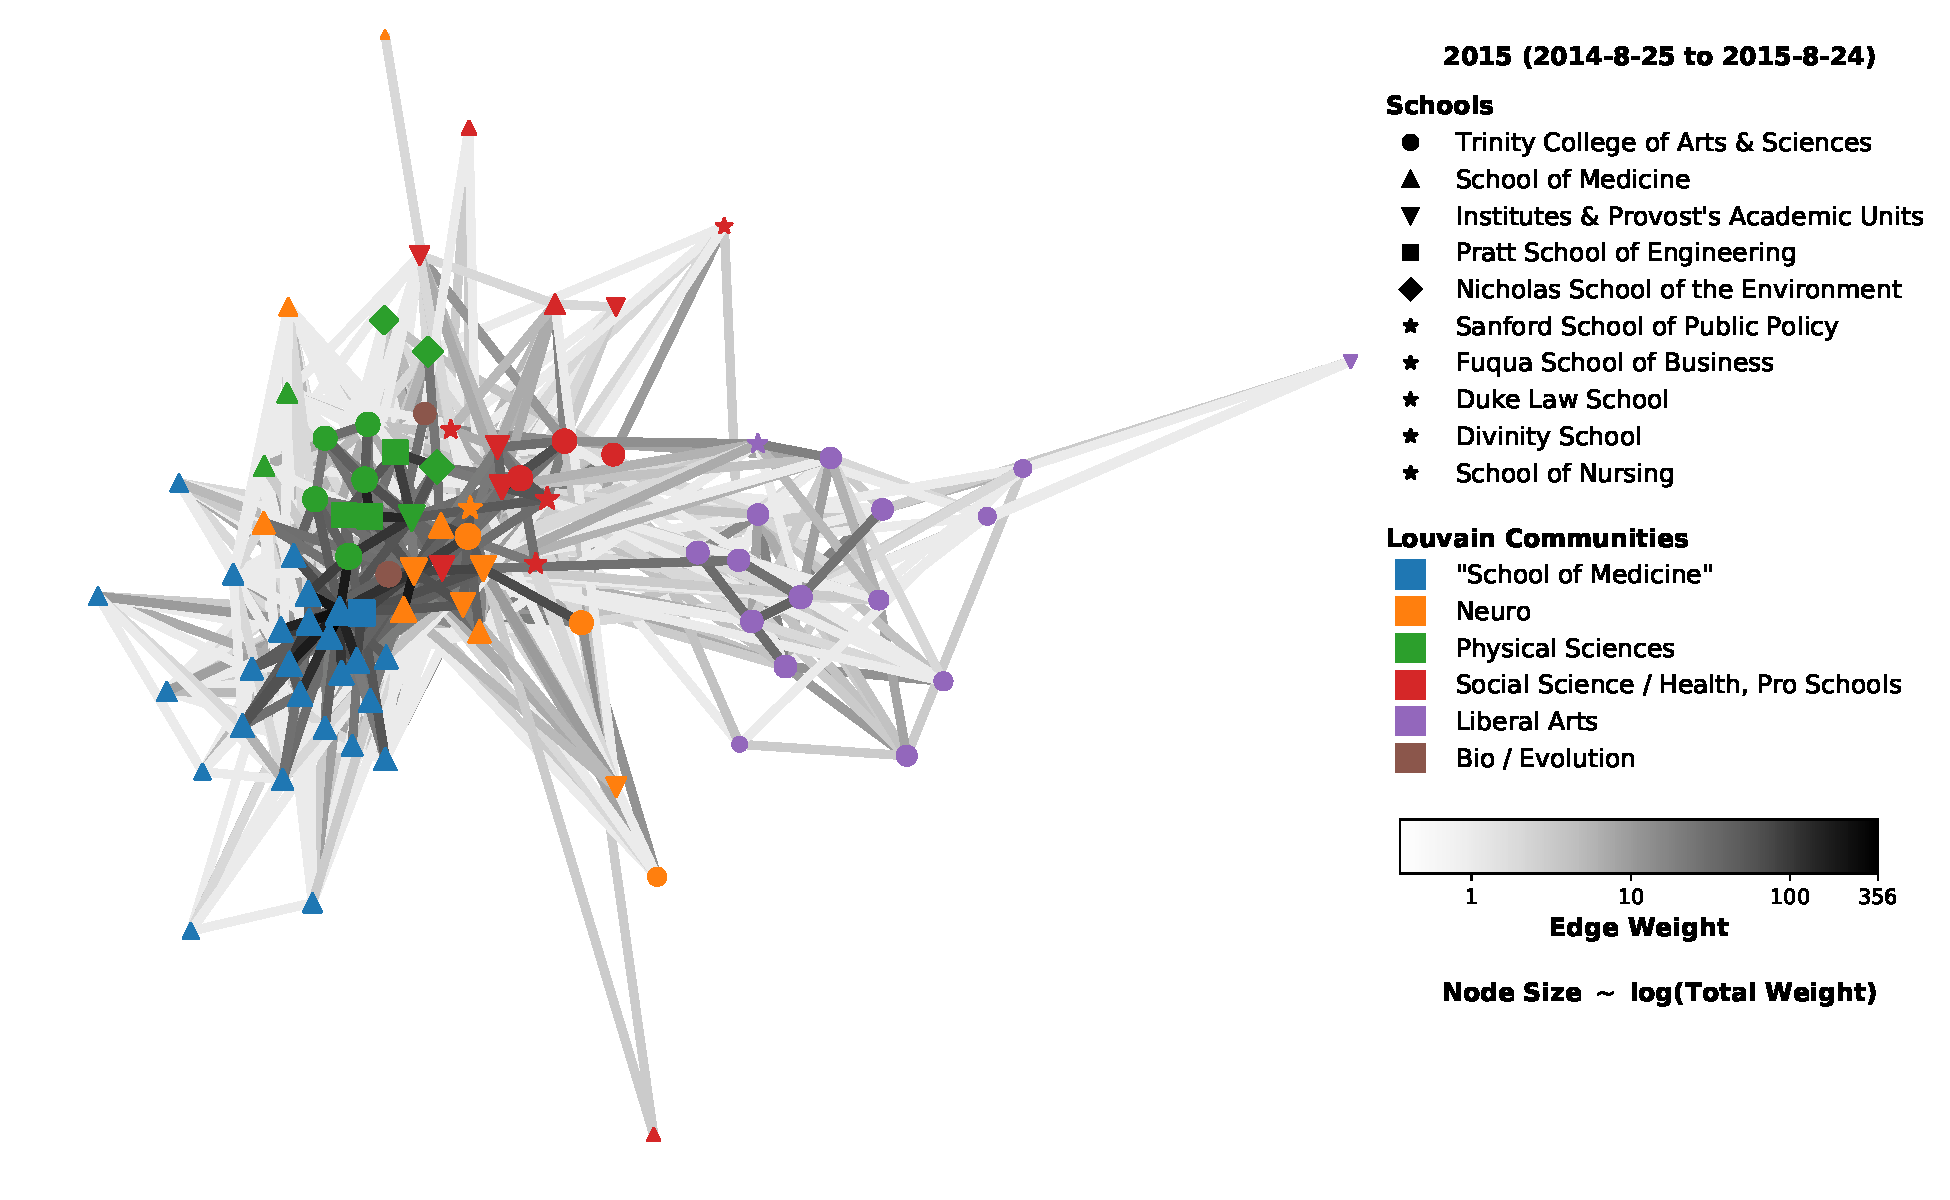
\includegraphics[width=\textwidth]{\figures/time_binned_networks/network_2015.pdf}
  \caption{Academic organizations graph for 2015.}
  % \label{fig:}
\end{figure}

% \vspace{0.15cm}
\begin{figure}[!htb]\centering
  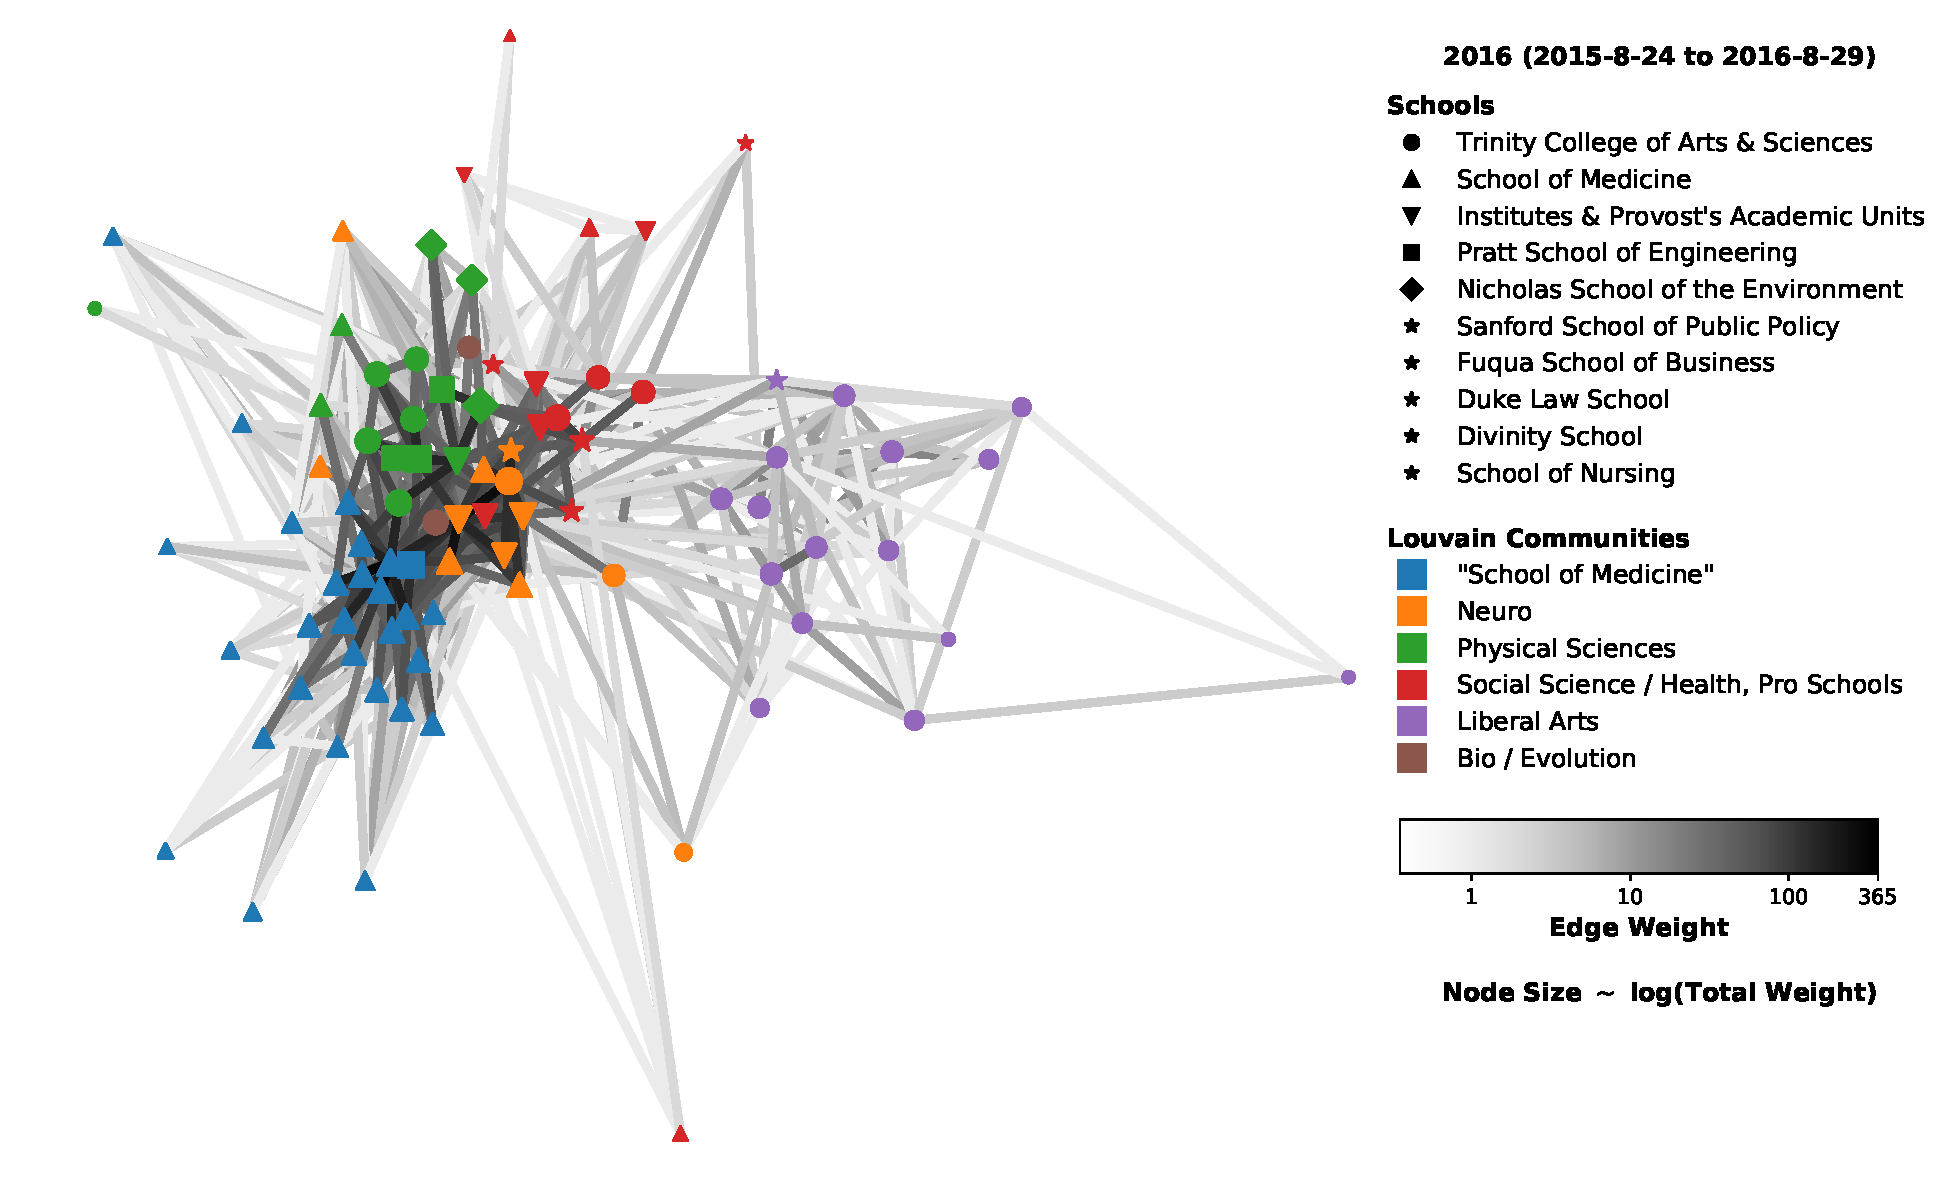
\includegraphics[width=\textwidth]{\figures/time_binned_networks/network_2016.pdf}
  \caption{Academic organizations graph for 2016.}
  % \label{fig:}
\end{figure}

% \vspace{0.15cm}
\begin{figure}[!htb]\centering
  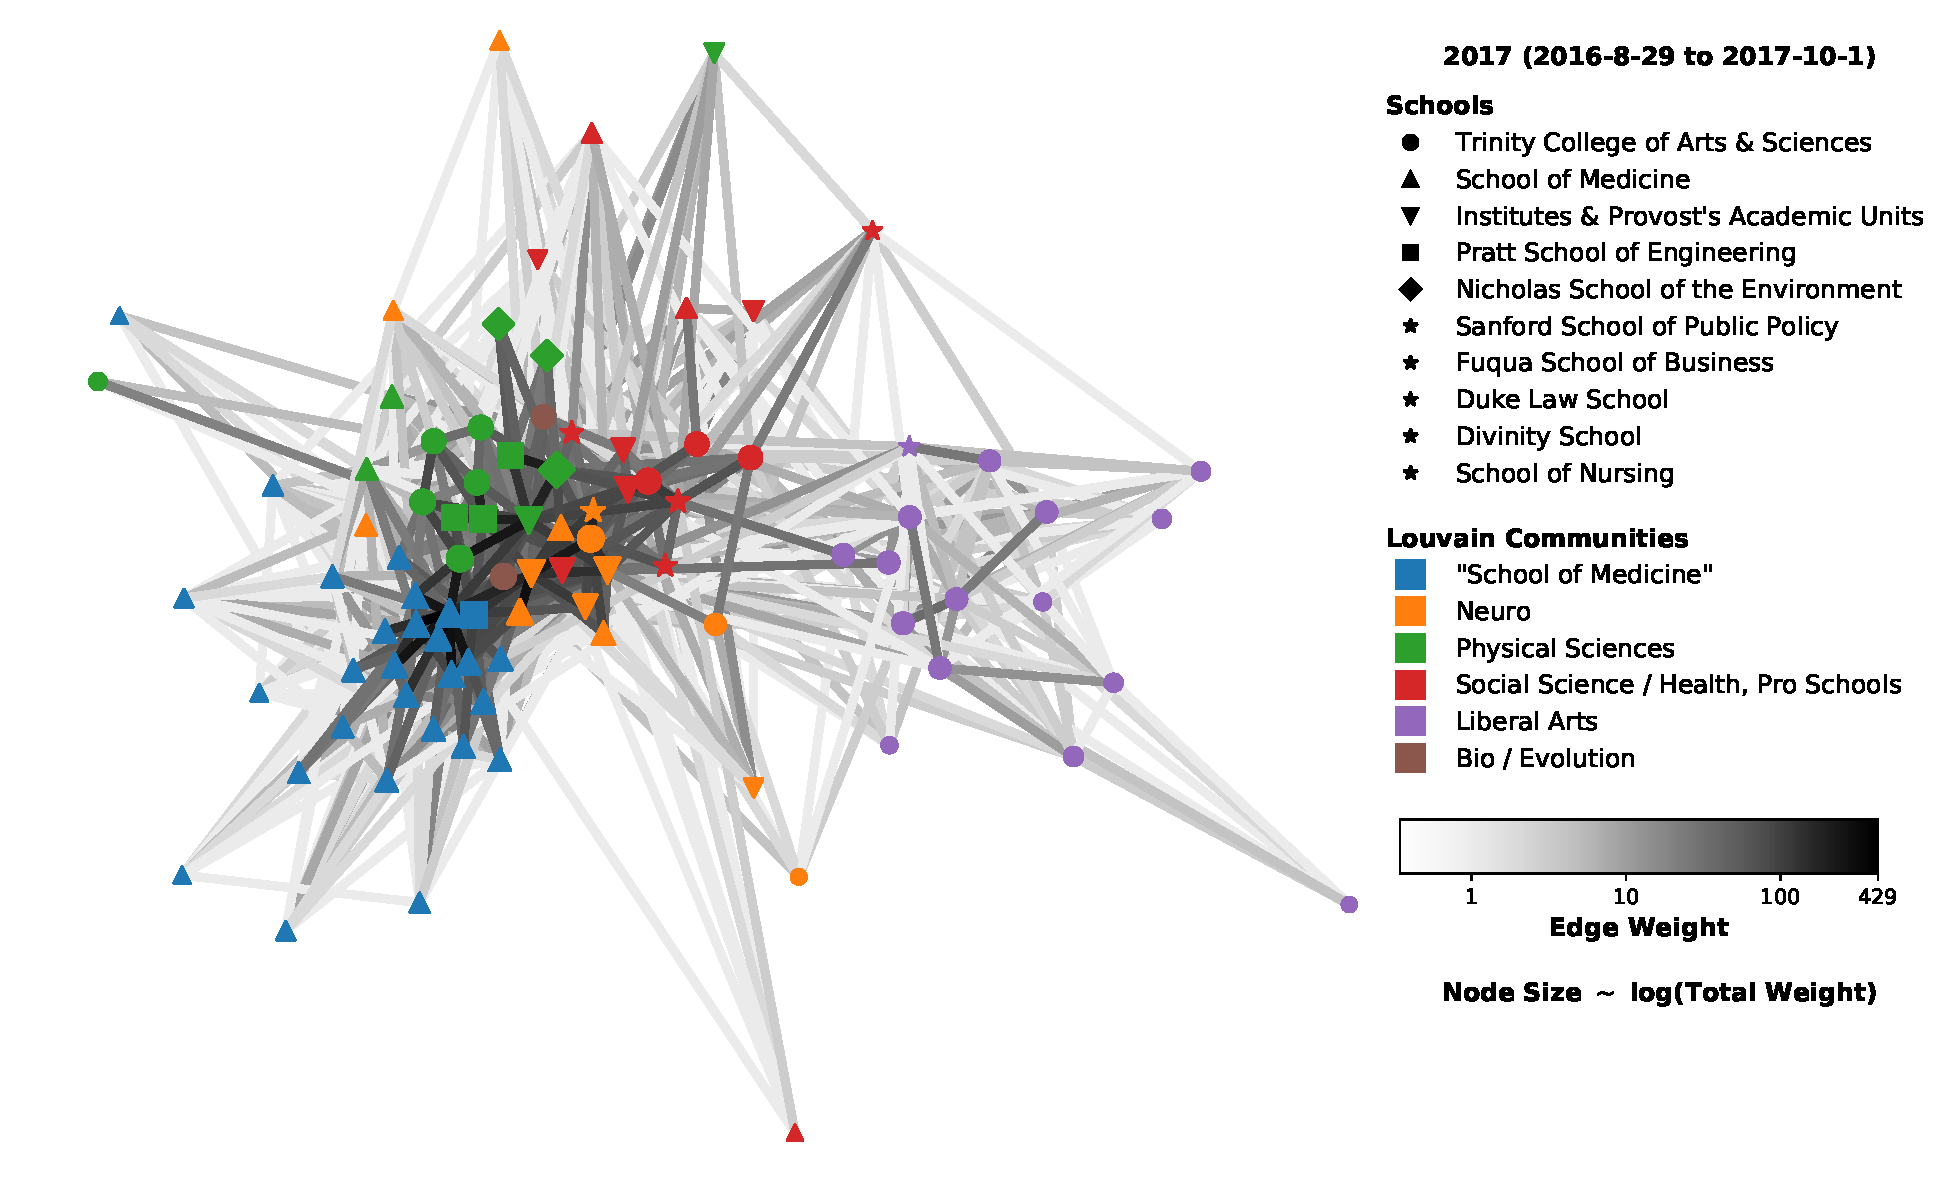
\includegraphics[width=\textwidth]{\figures/time_binned_networks/network_2017.pdf}
  \caption{Academic organizations graph for 2017.}
  % \label{fig:}
\end{figure}


\appendix*
\section{Interdisciplinary Fraction by Community}

% \vspace{0.15cm}
\begin{figure}[!htb]\centering
  \includegraphics[width=\textwidth]{\figures/interdis_frac/communities/School_of_Medicine.pdf}
  \caption{Interdisciplinary fraction vs year for the ``School of Medicine'' community.}
  % \label{fig:}
\end{figure}

% \vspace{0.15cm}
\begin{figure}[!htb]\centering
  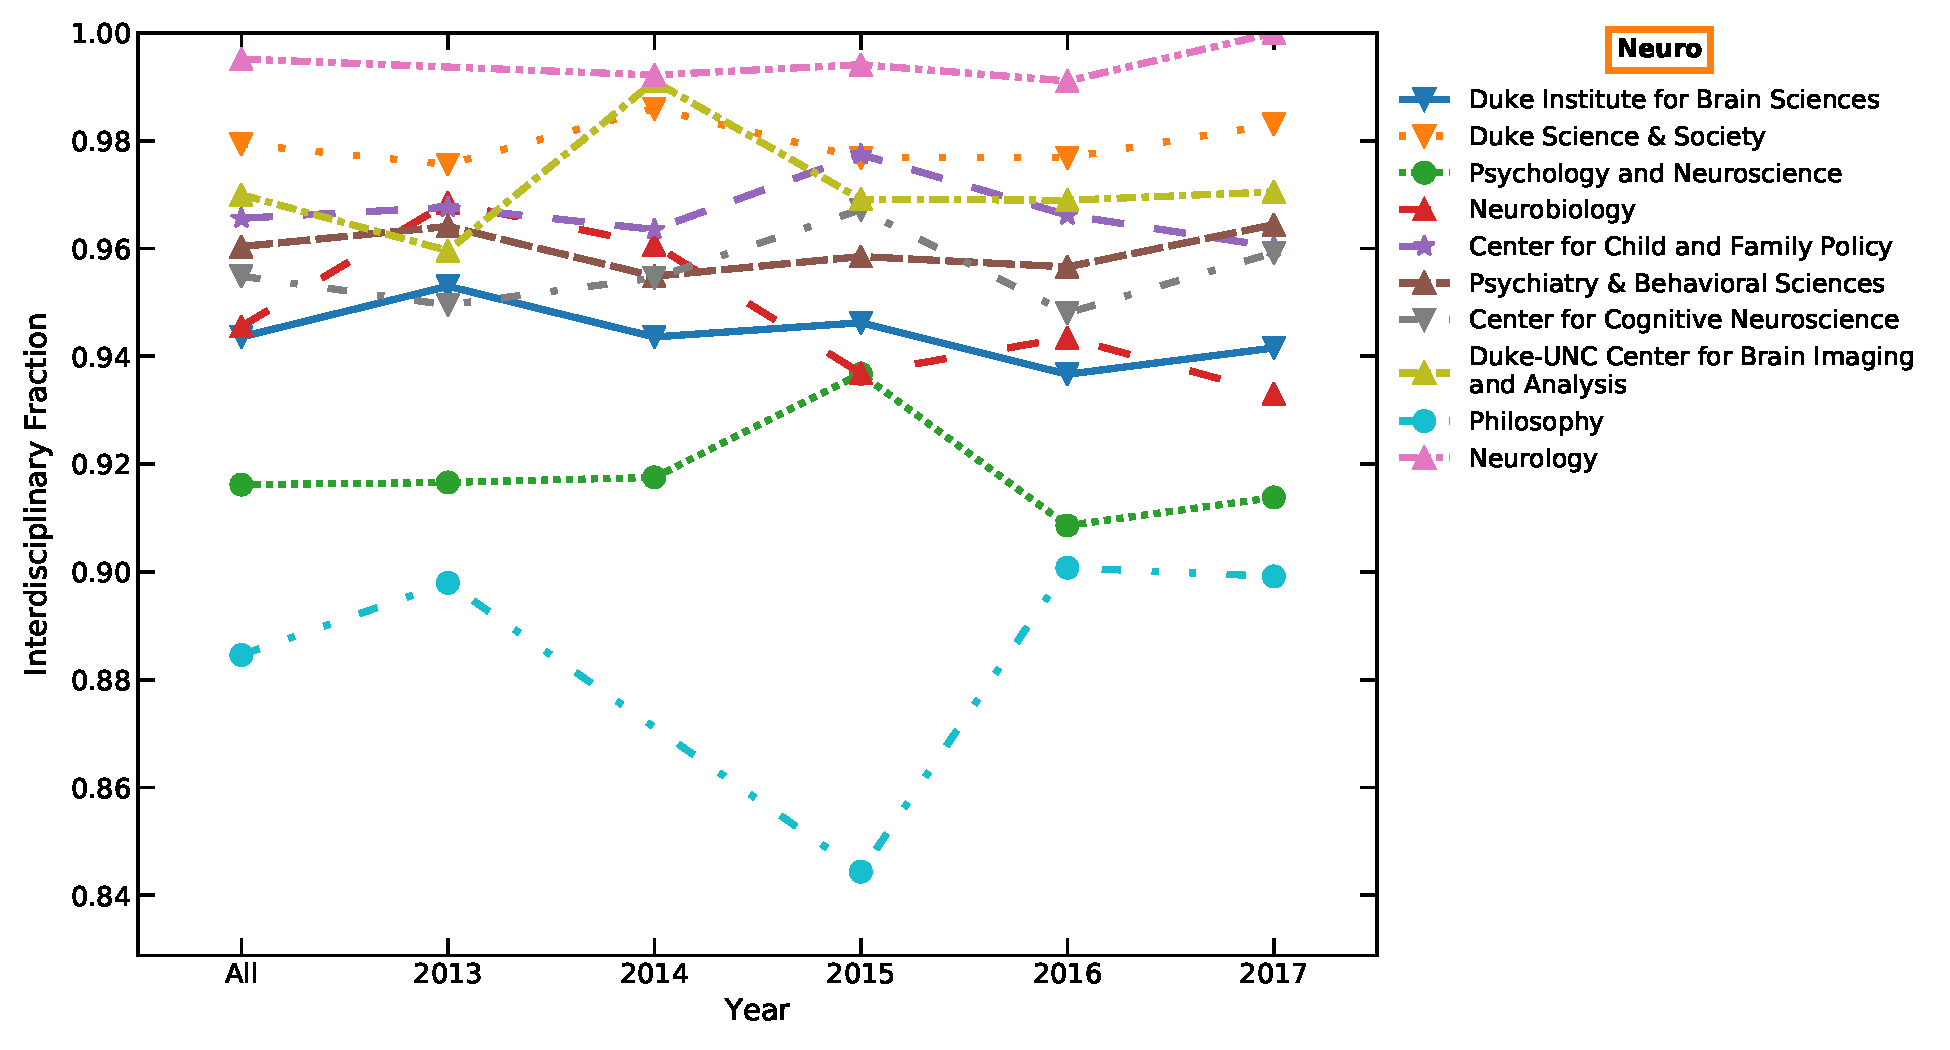
\includegraphics[width=\textwidth]{\figures/interdis_frac/communities/Neuro.pdf}
  \caption{Interdisciplinary fraction vs year for the Neuro community.}
  % \label{fig:}
\end{figure}

% \vspace{0.15cm}
\begin{figure}[!htb]\centering
  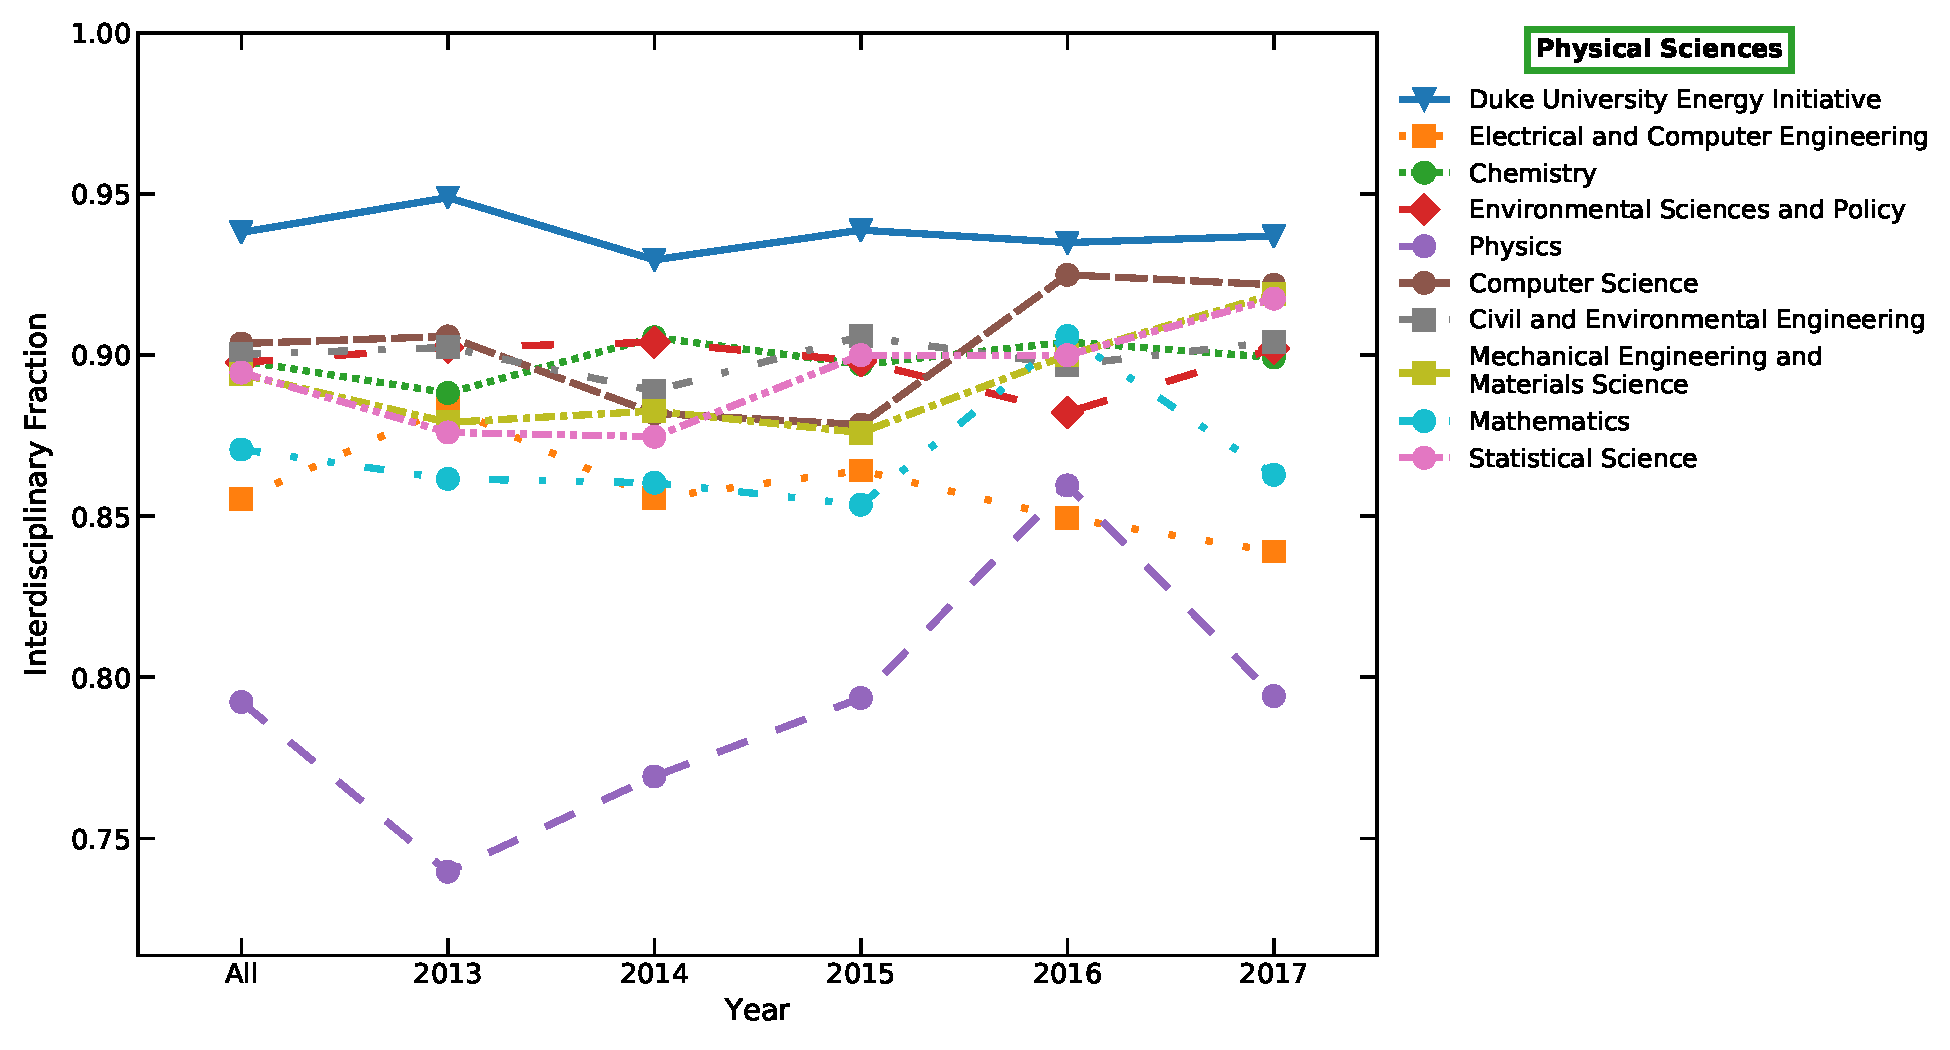
\includegraphics[width=\textwidth]{\figures/interdis_frac/communities/Physical_Sciences.pdf}
  \caption{Interdisciplinary fraction vs year for the Physical Sciences community.}
  % \label{fig:}
\end{figure}

% \vspace{0.15cm}
\begin{figure}[!htb]\centering
  \includegraphics[width=\textwidth]{\figures/interdis_frac/communities/Social_Science_slash_Health,_Pro_Schools.pdf}
  \caption{Interdisciplinary fraction vs year for the Social Science / Health, Pro Schools community.}
  % \label{fig:}
\end{figure}

% \vspace{0.15cm}
\begin{figure}[!htb]\centering
  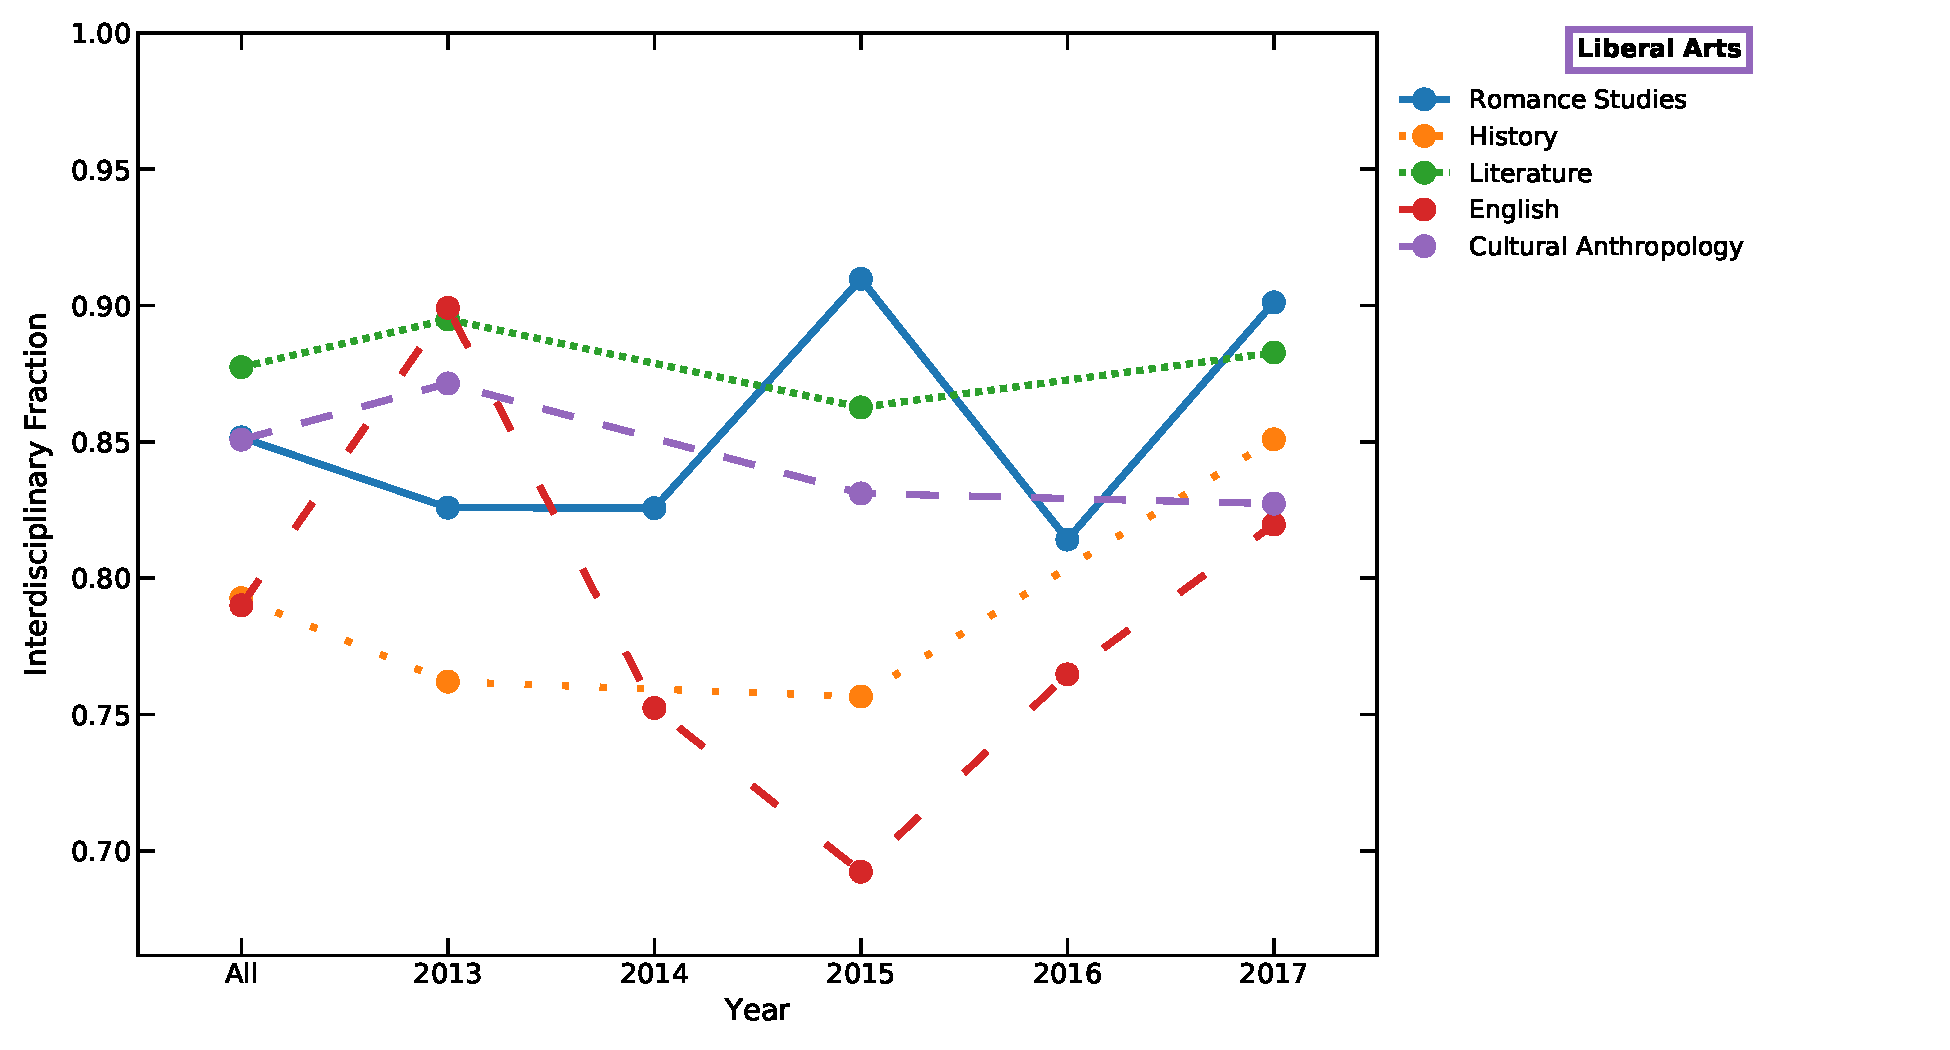
\includegraphics[width=\textwidth]{\figures/interdis_frac/communities/Liberal_Arts.pdf}
  \caption{Interdisciplinary fraction vs year for the Liberal Arts community.}
  % \label{fig:}
\end{figure}

% \vspace{0.15cm}
\begin{figure}[!htb]\centering
  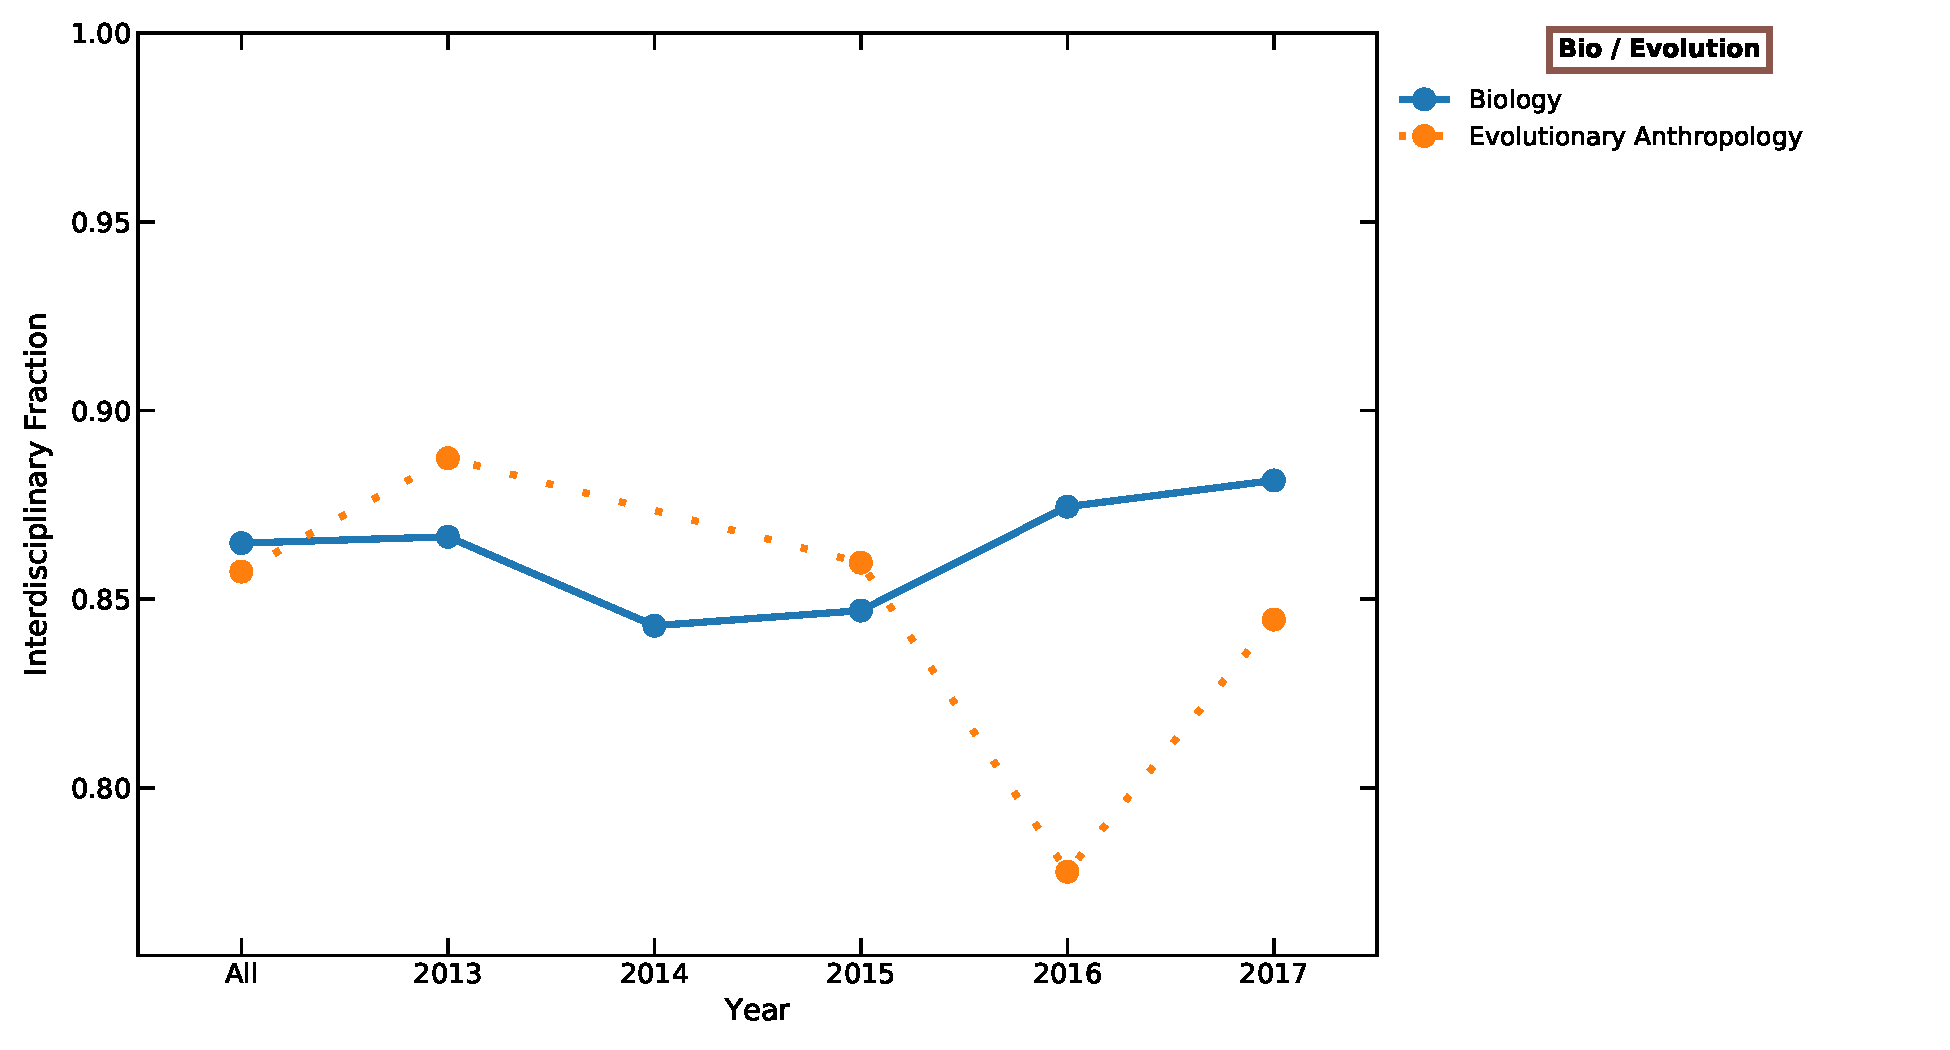
\includegraphics[width=\textwidth]{\figures/interdis_frac/communities/Bio_slash_Evolution.pdf}
  \caption{Interdisciplinary fraction vs year for the Bio / Evolution community.}
  % \label{fig:}
\end{figure}


\appendix*
\section{Interdisciplinary Fraction by School}

% \vspace{0.15cm}
\begin{figure}[!htb]\centering
  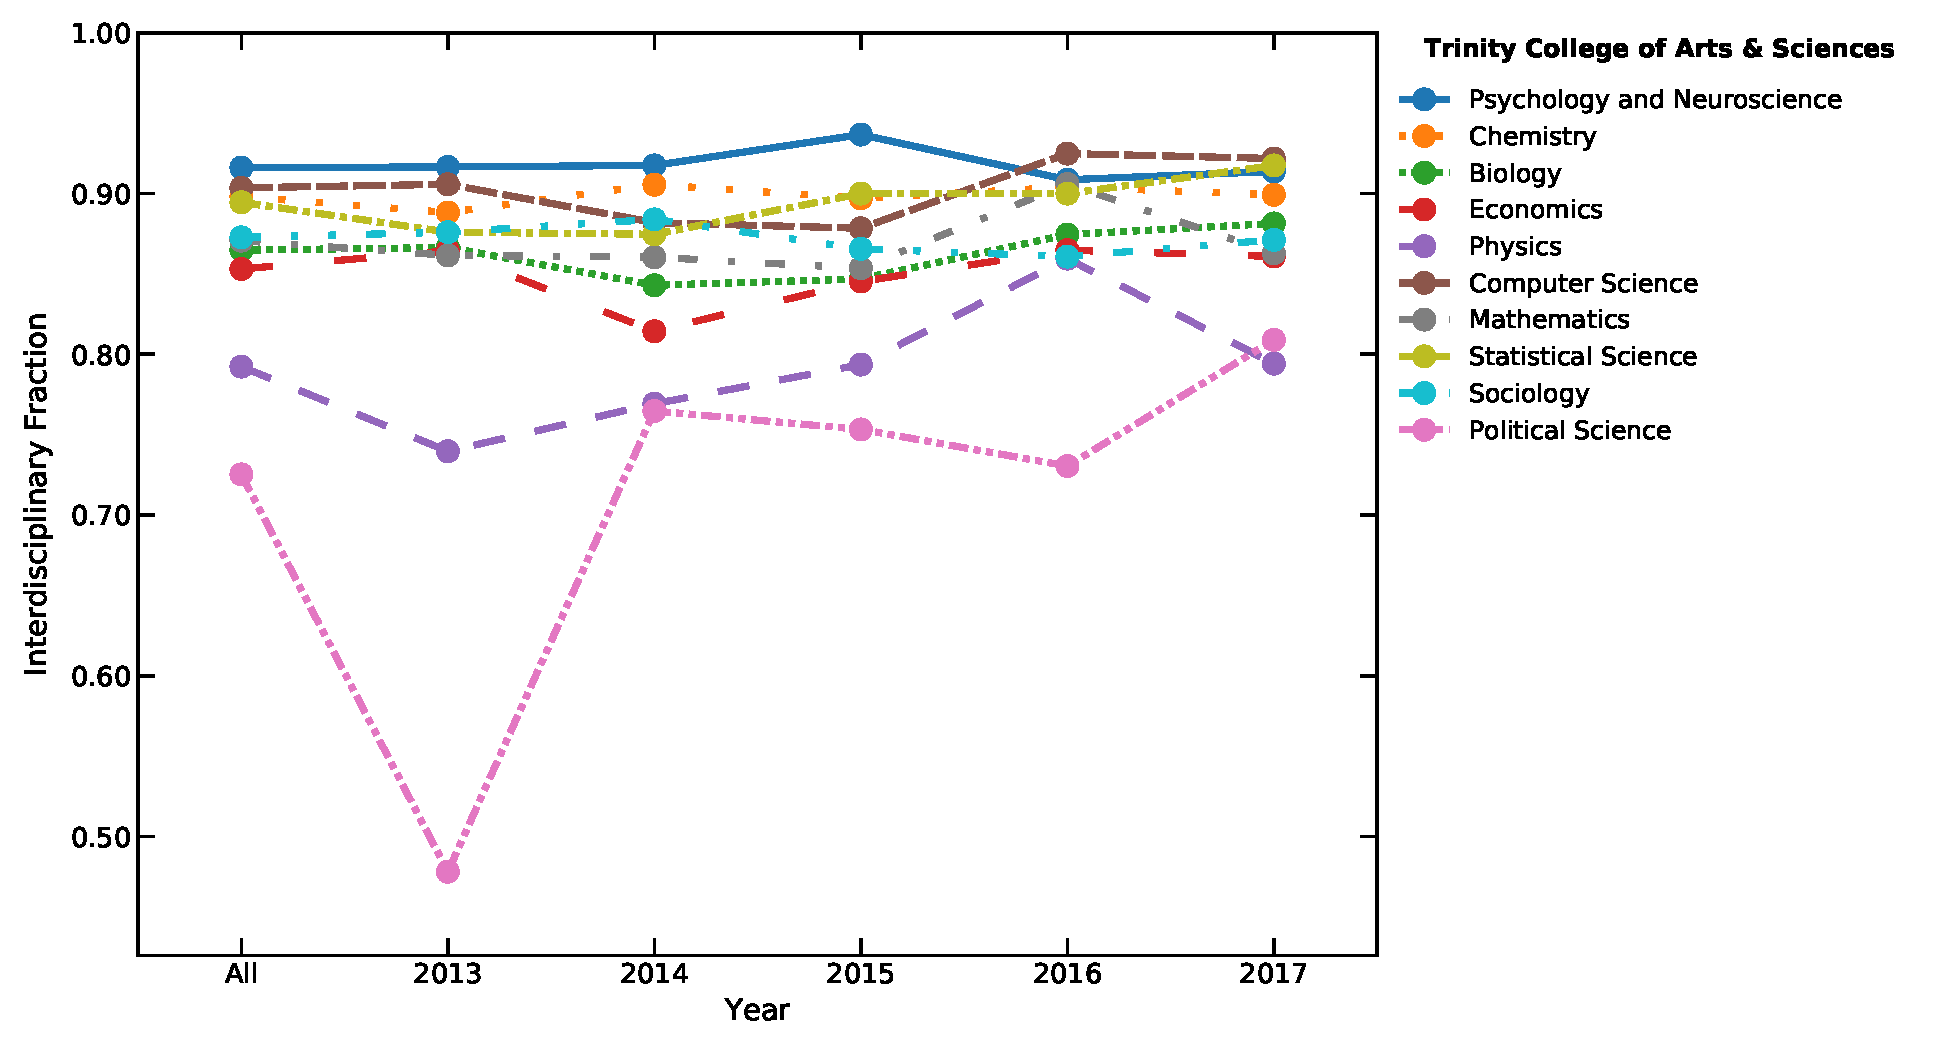
\includegraphics[width=\textwidth]{\figures/interdis_frac/schools/Trinity_College_of_Arts_and_Sciences.pdf}
  \caption{Interdisciplinary fraction vs year for the Trinity College of Arts \& Sciences.}
  % \label{fig:}
\end{figure}

% \vspace{0.15cm}
\begin{figure}[!htb]\centering
  \includegraphics[width=\textwidth]{\figures/interdis_frac/schools/School_of_Medicine.pdf}
  \caption{Interdisciplinary fraction vs year for the School of Medicine.}
  % \label{fig:}
\end{figure}

% \vspace{0.15cm}
\begin{figure}[!htb]\centering
  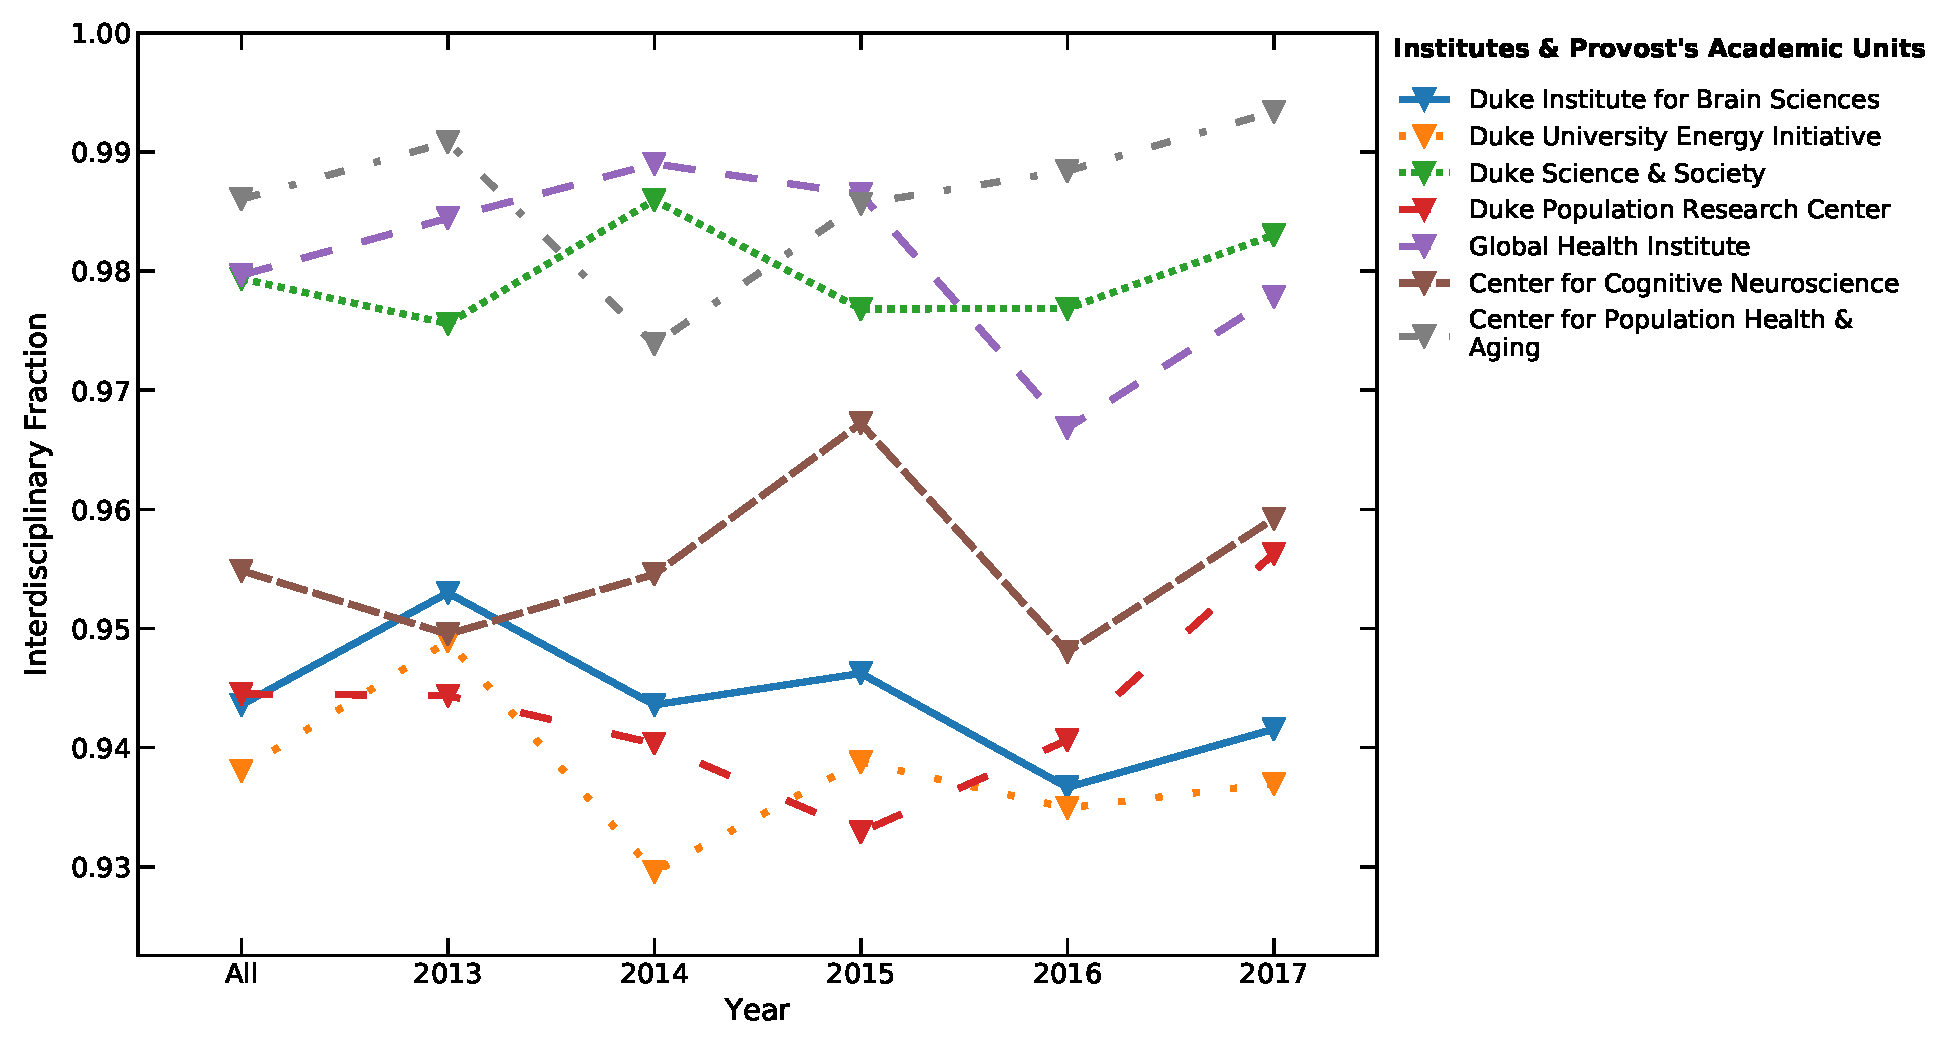
\includegraphics[width=\textwidth]{\figures/interdis_frac/schools/Institutes_and_Provosts_Academic_Units.pdf}
  \caption{Interdisciplinary fraction vs year for the Institutes \& Provost's Academic Units.}
  % \label{fig:}
\end{figure}

% \vspace{0.15cm}
\begin{figure}[!htb]\centering
  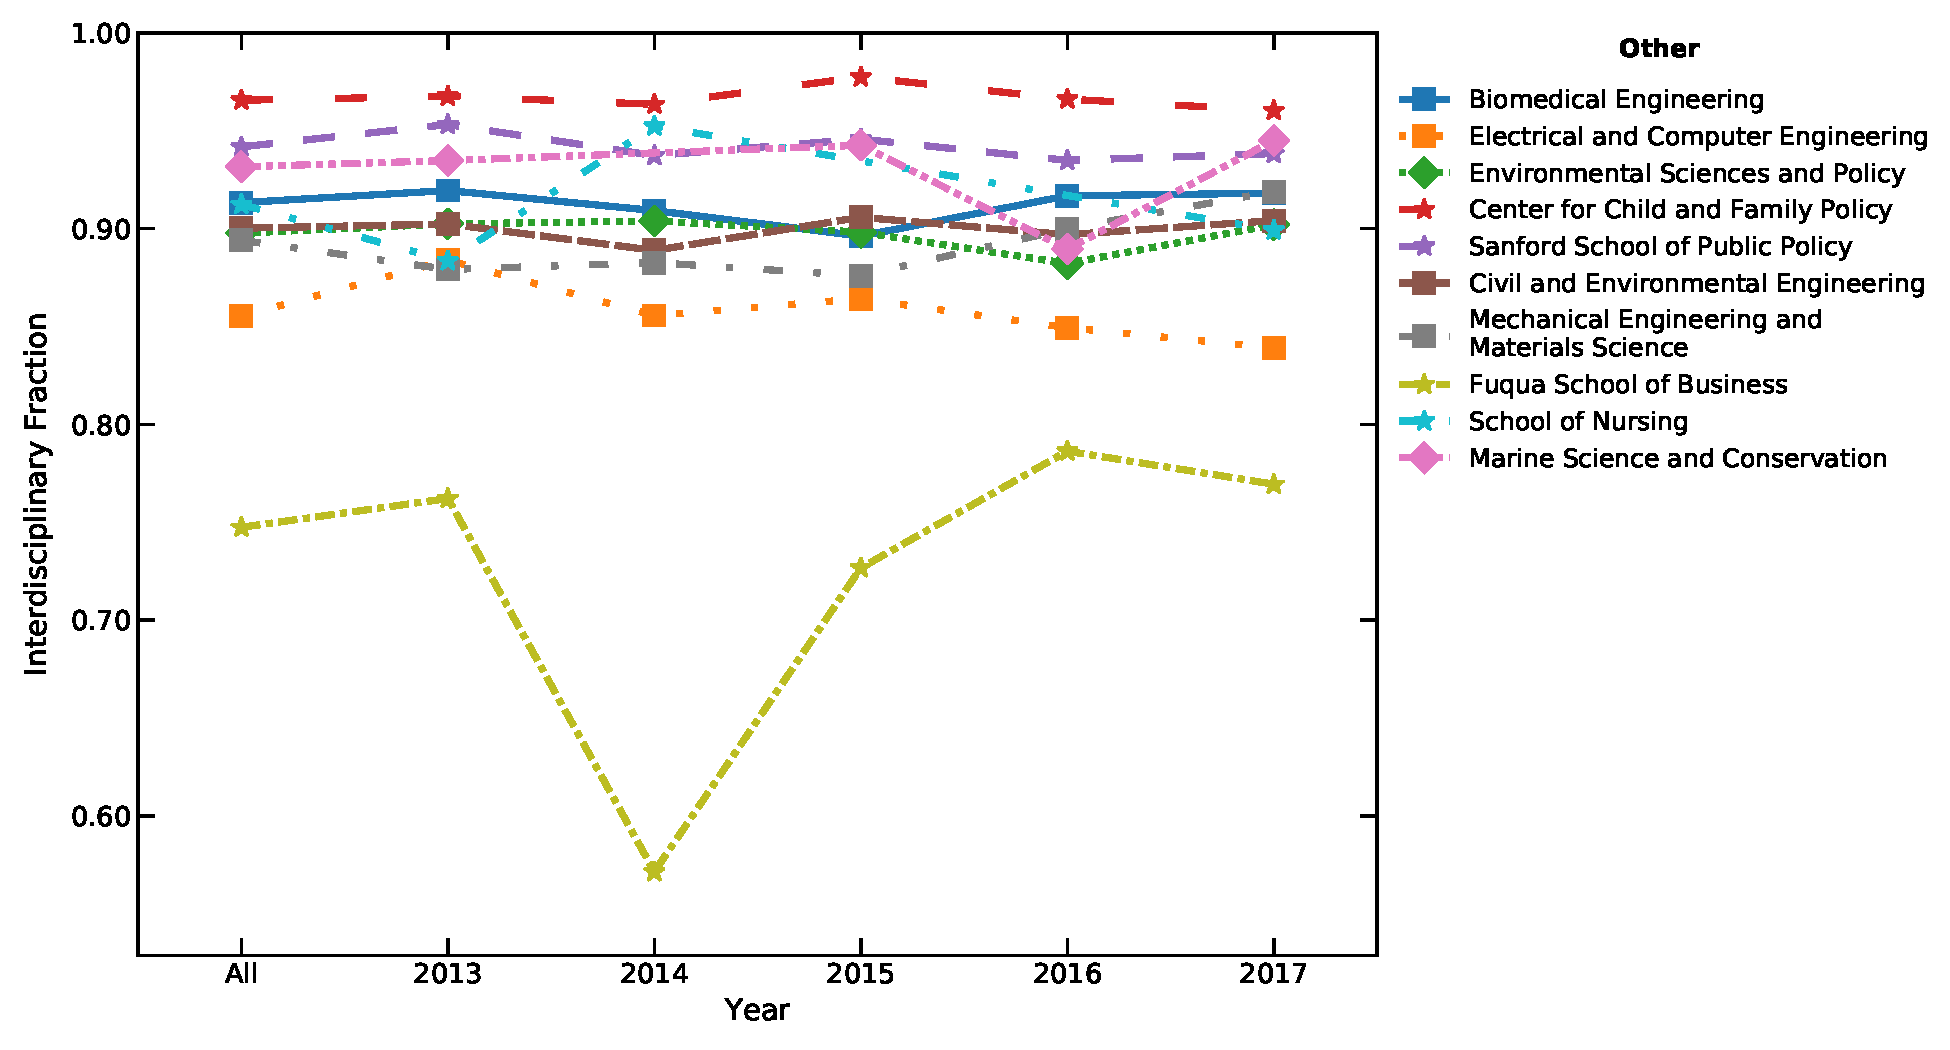
\includegraphics[width=\textwidth]{\figures/interdis_frac/schools/Other.pdf}
  \caption{Interdisciplinary fraction vs year for the remaining schools and units.}
  % \label{fig:}
\end{figure}

\end{document}
